%%%%%%%%%%%%%%%%%%%%%%%%%%%%%%%%%%%%%%%%%%%%%%%%%%%%%%%%%%%%%%%%%%%%%%%%%%%%%
%%%
%%% File: utthesis2.doc, version 2.0jab, February 2002
%%%
%%% Based on: utthesis.doc, version 2.0, January 1995
%%% =============================================
%%% Copyright (c) 1995 by Dinesh Das.  All rights reserved.
%%% This file is free and can be modified or distributed as long as
%%% you meet the following conditions:
%%%
%%% (1) This copyright notice is kept intact on all modified copies.
%%% (2) If you modify this file, you MUST NOT use the original file name.
%%%
%%% This file contains a template that can be used with the package
%%% utthesis.sty and LaTeX2e to produce a thesis that meets the requirements
%%% of the Graduate School of The University of Texas at Austin.
%%%
%%% All of the commands defined by utthesis.sty have default values (see
%%% the file utthesis.sty for these values).  Thus, theoretically, you
%%% don't need to define values for any of them; you can run this file
%%% through LaTeX2e and produce an acceptable thesis, without any text.
%%% However, you probably want to set at least some of the macros (like
%%% \thesisauthor).  In that case, replace "..." with appropriate values,
%%% and uncomment the line (by removing the leading %'s).
%%%
%%%%%%%%%%%%%%%%%%%%%%%%%%%%%%%%%%%%%%%%%%%%%%%%%%%%%%%%%%%%%%%%%%%%%%%%%%%%%

%%%%%%%%%%%%%%%%%%%%%%%%%%%%%%%%%%%%%%%%%%%%%%%%%%%%%%%%%%%%%%%%%%%%%%%%%%%%%
%%%
%%
%% This file, and the corresponding tcdthesis.sty the accompanied it, have
%% been modified for the M.Sc. styles used in Trinity College, Dublin
%%
%%
%%%%%%%%%%%%%%%%%%%%%%%%%%%%%%%%%%%%%%%%%%%%%%%%%%%%%%%%%%%%%%%%%%%%%%%%%%%%%
\documentclass[a4paper, 12pt, oneside]{report}         %% LaTeX2e document.
\usepackage {tcdthesis}              %% Preamble.

\mastersthesis                       %% Uncomment one of these; if you don't
% \phdthesis                         %% use either, the default is \phdthesis.

\thesisdraft                         %% Uncomment this if you want a draft
                                     %% version; this will print a timestamp
                                     %% on each page of your thesis.

\leftchapter                         %% Uncomment one of these if you want
% \centerchapter                     %% left-justified, centered or
% \rightchapter                      %% right-justified chapter headings.
                                     %% Chapter headings includes the
                                     %% Contents, Acknowledgments, Lists
                                     %% of Tables and Figures and the Vita.
                                     %% The default is \centerchapter.

% \singlespace                       %% Uncomment one of these if you want
\oneandhalfspace                     %% single-spacing, space-and-a-half
% \doublespace                       %% or double-spacing; the default is
                                     %% \oneandhalfspace, which is the
                                     %% minimum spacing accepted by the
                                     %% Graduate School.

\renewcommand{\thesisauthor}{Maxime Mu}                %% Your official TCD name.
\renewcommand{\thesismonth}{August}                   %% Your month of graduation.
\renewcommand{\thesisyear}{2024}                      %% Your year of graduation.
\renewcommand{\thesistitle}{Generating Synthetic Data using Large Language Models}          %% The title of your thesis; use mixed-case.
\renewcommand{\thesisauthorpreviousdegrees}{, BAI}    %% Your previous degrees, abbreviated; separate multiple degrees by commas.
\renewcommand{\thesissupervisor}{Tin Lok James Ng}            %% Your thesis supervisor; use mixed-case and don't use any titles or degrees.
% \renewcommand{\thesiscosupervisor}{}                %% Your PhD. thesis co-supervisor; if any.

% \renewcommand{\thesiscommitteemembera}{}
% \renewcommand{\thesiscommitteememberb}{}
% \renewcommand{\thesiscommitteememberc}{}
% \renewcommand{\thesiscommitteememberd}{}
% \renewcommand{\thesiscommitteemembere}{}
% \renewcommand{\thesiscommitteememberf}{}
% \renewcommand{\thesiscommitteememberg}{}
% \renewcommand{\thesiscommitteememberh}{}
% \renewcommand{\thesiscommitteememberi}{}


\renewcommand{\thesisauthoraddress}{.......}

\renewcommand{\thesisdedication}{...}     %% Your dedication, if you have one; use "\\" for linebreaks.


%%%%%%%%%%%%%%%%%%%%%%%%%%%%%%%%%%%%%%%%%%%%%%%%%%%%%%%%%%%%%%%%%%%%%%%%%%%%%
%%%
%%% The following commands are all optional, but useful if your requirements
%%% are different from the default values in tcdthesis.sty.  To use them,
%%% simply uncomment (remove the leading %) the line(s).

\renewcommand{\thesisdegree}{Master of Science in Computer Science}
                                     %% default is "DOCTOR OF PHILOSOPHY"
                                     %% for \phdthesis or "MASTER OF ARTS"
                                     %% for \mastersthesis.  Provide the
                                     %% correct FULL OFFICIAL name of
                                     %% the degree.
\renewcommand{\thesisdegreestream}{ (Intelligent Systems)}
                                     %% Default is empty. This is used on
                                     %% the title page of the thesis.

\renewcommand{\thesisdegreeabbreviation}{M.Sc.}
                                     %% Use this if you also use the above
                                     %% command; provide the OFFICIAL
                                     %% abbreviation of your thesis degree.
\renewcommand{\thesistype}{Dissertation}    %% Use this ONLY if your thesis type
                                     %% is NOT "Thesis" for \phdthesis
                                     %% or \mastersthesis.
                                     %% Provide the OFFICIAL type of the
                                     %% thesis; use mixed-case.

%%%
%%%%%%%%%%%%%%%%%%%%%%%%%%%%%%%%%%%%%%%%%%%%%%%%%%%%%%%%%%%%%%%%%%%%%%%%%%%%%

\usepackage{graphicx,color}
\usepackage{anysize}
\usepackage{amsmath}
\usepackage{natbib}
\usepackage{caption}
\usepackage{subcaption}
\usepackage{hyperref}
\usepackage{listings}
\usepackage{float}
\usepackage{array}
\usepackage{booktabs}
\usepackage{tabularx}
\usepackage{makecell}
\usepackage{adjustbox}
\usepackage{tikz}
\usetikzlibrary{positioning}


%%------------------------------------------------
%% Listing macros
%%------------------------------------------------
%% Examples for the commands in the document below
%%
%% includecode:
%% \includecode{caption for table of listings}{caption for reader}{filename}
%% - includes a file with code and adds a caption that should describe the code in some detail and a shorter caption for the table of listings
\newcommand{\includecode}[4]{\lstinputlisting[floatplacement=H, caption={[#1]#2}, captionpos=b, frame=single, label={#3}]{#4}}

%%------------------------------------------------
%% Image macros
%%------------------------------------------------

%% includescalefigure:
%% \includescalefigure{label}{short caption}{long caption}{scale}{filename}
%% - includes a figure with a given label, a short caption for the table of contents and a longer caption that describes the figure in some detail and a scale factor 'scale'
\newcommand{\includescalefigure}[5]{
\begin{figure}[htb]
\centering
\includegraphics[width=#4\linewidth]{#5}
\captionsetup{width=.8\linewidth} 
\caption[#2]{#3}
\label{#1}
\end{figure}
}

%% includefigure:
%% \includefigure{label}{short caption}{long caption}{filename}
%% - includes a figure with a given label, a short caption for the table of contents and a longer caption that describes the figure in some detail
\newcommand{\includefigure}[4]{
\begin{figure}[htb]
\centering
\includegraphics{#4}
\captionsetup{width=.8\linewidth} 
\caption[#2]{#3}
\label{#1}
\end{figure}
}





\begin{document}                                  %% BEGIN THE DOCUMENT

\thesistitlepage                                  %% Generate the title page.

%\hypersetup{pageanchor=false}
%\thesisdeclarationpage                            %% Generate the declaration page.

%\thesispermissionpage                             %% Generate the copyright permission page
%\hypersetup{pageanchor=true}

\begin{thesisabstract}                            %% the abstract for your thesis
...ABSTRACT...
\end{thesisabstract}

%\thesisdedicationpage                            %% Generate the dedication page.

\begin{thesisacknowledgments}                     %% Use this to write your
  Thank you Mum \& Dad.                           %% acknowledgments; it can be anything
\end{thesisacknowledgments}                       %% allowed in LaTeX2e par-mode.
  
  
\tableofcontents                                  %% Generate table of contents.
\listoftables                                     %% Uncomment this to generate list of tables.
\listoffigures                                    %% Uncomment this to generate list of figures.


%%
%% Include thesis chapters here...
%%
\chapter{Introduction}


%%%%%%%%%%%%%%%%%%%%%%%% INTRODUCTION %%%%%%%%%%%%%%%%%%%%%%

The rapid progress of technology tools has tremendously increased new opportunities for simplifying manual tasks. Numerous fields have started to adopt this approach as people have seen the potential. In fact, one of the most innovative tools that has been used in our everyday lives is tabular data. At first sight, we don't realise how deeply ingrained it is in our daily routines. From the spreadsheets people use for managing finance-related tasks to the train schedules we consult, tabular data silently underpins countless interactions in our daily lives. 

\section{What is a Synthetic Data ?}
\label{sec:DefinitionSyntheticData}

%%%%%%%%%%%%%%%%%%% DEFINITION %%%%%%%%%%%%%%%%%%%%%%%%%%%%%%
Tabular data is well-structured data arranged as a table where each row represents an individual record or observation and each column represents a specific variable or feature associated with that record. It has been widely adopted as it offers numerous advantages that facilitate data manipulation and reading. Nowadays, the most commonly used formats for representing tabular data are CSV (Comma-Separated Values) and XLS (specific format in Microsoft Excel software). The difference between the two mentioned formats is that a CSV file is lightweight compared to XLS as a CSV file is mainly defined as a plain text file that can be easily read and processed by any program. Conversely, XLS is formatted as a compressed binary file and requires specific software to read the file content. However, XLS offers a wide range of data analytics features that CSV does not support such as data manipulation with formulas, charts and pivot tables.

%%%%%%%%%%%%%%%%% DIFFERENCE %%%%%%%%%%%%%%%%%%%%%%%%%%%%%%%%
\vspace{0.5cm}
The relation between a dataset and tabular data is that tabular data is a way of arranging data within a dataset. As a matter of fact, a dataset can be in various formats such as text files, images, and tables. Tabular formatting showed its efficiency in its widespread adoption for data analysis and machine learning tasks. For example, Kaggle, a popular platform referencing all datasets from various domains from healthcare to finance data, utilises a tabular format. 

%%%%%%%%%%%%%%%%% PYTHON %%%%%%%%%%%%%%%%%%%%%%%%%%%%%%%%%%%
\vspace{0.5cm}
Programming languages like Python offer powerful libraries, such as pandas, that make tabular data reading and manipulation incredibly efficient. Other languages such as R and Java also provide robust libraries for working with tabular data, Python remains the most used programming language for tabular data considering its potential domain of applications.

\section{Importance in the Healthcare Domain}
\label{sec:healthcare}

This paper delves deeper into the healthcare domain, specifically focusing on hospital patient records. Patient health records can be efficiently organised in a tabular format as each row represents an individual patient, with each column capturing different aspects of their health such as their age, names, diagnoses, medications, or treatment history. 

%%%%%%%%%%%%%%%%%%%% CHALLENGE %%%%%%%%%%%%%%%%%%%%%%%%%%%
\vspace{0.5cm}
However, conducting a study on patients' data can prove quite challenging. In fact, not only the ethical question but also the security question pose a crucial problem as hospitals would easily not let anyone have access to their patient's records and the increase in the number of data tends to increase the probability of security and privacy breaches (\cite{Abouelmehdi2018}). Patient data is considered very sensitive as it contains personal information about each patient. Hospitals have been for many years targets of cyberattacks. Hackers try to get access to sensitive data and ask for a ransom from hospitals as they could potentially expose sensitive data and compromise patient privacy leading to identity theft and disruptions in critical care. For example, in the \cite{Abouelmehdi2018} paper, over 3 million patient records have been breached in one year, and 40\% of breach incidents are due to unauthorized access/disclosure. The high risks and consequences mentioned above undeniably impose a major constraint on the number of possible studies and research projects within the healthcare domain (\cite{DataSynthesizer2017}, \cite{ElEmam2020}). 

%%%%%%%%%%%%%%%%%%%%% RESEARCH %%%%%%%%%%%%%%%%%%%%%%%%%%%%%%
\vspace{0.5cm}
Research is fundamental as it drives disease diagnosis and treatment advancements, leading to more effective medication development and personalised and faster treatments (\cite{Abouelmehdi2018}). Additionally, research could help us understand the progression of diseases, identify risk factors, and develop preventative measures.

%%%%%%%%%%%%%%%%%%% SYNTHETIC DATA %%%%%%%%%%%%%%%%%%%%%%%%%
\vspace{0.5cm}
This is where synthetic data comes into play. With an increasing interest in synthetic data usage, it refers to artificially generated data that mimic properties and statistical characteristics of real-world data but does not contain any real information (\cite{ElEmam2020}). This means fictional patient records can be synthesized without having real information about patients on the fictional data, which can be artificial enough to reassure data owners and provide robust privacy safeguards to prevent adversaries from extracting sensitive information (\cite{DataSynthesizer2017}). Synthetic data is a huge boon for ethical and privacy-conscious research, this suggests scientists can explore new possibilities and conduct experiments without compromising patient confidentiality. As a matter of fact, synthetic data could help hospitals determine even faster symptoms from future patients and treat the patient's disease more effectively and, overall, with possibly less cost.

\section{Limitations of Data Sources}
\label{sec:LimitationsTraditionalData}

Data sources in the healthcare field, such as patients' health records, have limitations that affect the data quality; a necessary factor if we want to conduct any data analysis or machine learning techniques. The patient's health records can sometimes be incomplete due to human error, a lack of standardisation in data entry, or a software error. The incompleteness of information represents a huge constraint for both hospitals and scientists. In hospitals, any missing or error in patients' records could lead to irreversible consequences to patients such as a patient being treated with the wrong medication.

\vspace{0.5cm}
Moreover, tracking the patient in the long term is difficult as the patient might resort to other health services. For example, the patient could switch to a different provider or insurer or they could have gone to another country.

\vspace{0.5cm}
These limitations make the current data in the healthcare domain very limited making it difficult for researchers and healthcare professionals to perform comprehensive data analysis.



\section{Existing State-of-the-Art Approaches in Generating Synthetic Data}
\label{sec:ExistingStateOfTheArtApproaches}

Several state-of-the-art approaches exist in generating synthetic data. Models like Generative Adversarial Networks (GANs) and Variational Autoencoders (VAEs) are examples.



\section{Large Language Models as a Powerful Tool for Generating Synthetic Data}
\label{sec:IntroductionLLMs}

%%%%%%%%%%%%%%%%%%%% LLM DEFINITION %%%%%%%%%%%%%%%%%%%%%%%%%%
Large Language Models (LLMs) have emerged as a powerful tool for generating synthetic data based on the user request. A LLM is a form of artificial intelligence algorithm trained on numerous large datasets encompassing a wide range of topics and linguistic features. They are capable of generating texts based on what the user asks for, thus they are also capable of producing relevant information that mimics real-world data. 

\vspace{0.5cm}
%%%%%%%%%%%%%%%%% EXAMPLES OF APPLICATION %%%%%%%%%%%%%%%%%%%%
They can be used, in particular, for data augmentation, which can augment existing patient datasets allowing researchers and healthcare professionals to conduct more comprehensive studies.
Additionally, they are used for bias mitigation which helps mitigate biases present in traditional datasets. For example, they can generate data that balances underrepresented patient populations, resulting in a more representative way of conducting experiments and analysis.
They also keep patients' data private as synthetic data does not correspond to real individuals' data. Thus, LLMs can address privacy concerns and compliance with regulations like HIPPA. This means that researchers can perform scientific analysis and experiments on the synthetic data without needing to worry about patient confidentiality.

One another aspect that LLMs can provide is creating scenarios. In fact, it is possible to imagine scenarios where bad events such as pandemics could happen so healthcare professionals and researchers know how to cure and act in the most efficient way. This could also allow for training medical students and professionals, allowing them to practice diagnosing and treating various hypothetical cases in a risk-free environment.


\section{Existing Research on LLMs for Data Generation}
\label{sec:ExisitingResearchLLMs}

% Briefly reviews existing research on LLMs for data generation.

LLMs offer various benefits that make it possible to generate realistic synthetic data. 

\begin{itemize}
    \item[1.] \textsc{Versatility and flexibility}\\
    LLMs can generate data for diverse fields such as healthcare, finance, marketing, and more. Thus, making them suitable for generating data in the healthcare domain. They can produce responses in a specific format and multiple languages. Additionally, they can change the writing style and tone of how sentences are formulated, thus resulting in more personalised information.

    \item[2.] \textsc{Quality}\\
    LLMs can provide relatively high-quality data depending on how well they perform. As a matter of fact, they are trained on several billion parameters; the more parameters the model is trained, the better the model will perform. LLMs trained on several billion parameters can grasp the context over long passages resulting in coherent accurate data. 

    \item[3.] \textsc{Scalability}\\
    LLMs can process very long requests and quickly produce a large volume of data. 

    \item[4.] \textsc{Ethical and privacy considerations}\\
    LLMs help generate data that mitigate privacy concerns by providing anonymized data. Researchers can use the generated data to study.

\end{itemize}

\chapter{Literature Review}


\section{Why is Tabular Data So Important ?}
\label{sec:whytabularsoimportant}

\subsection{Tabular is Used Everywhere}

Tabular data has been increasingly used for data formatting in the context of machine learning (ML), computer vision and data analysis (\cite{Lautrup2024}) as it allows for easy data manipulation and organisation; enabling computers to understand and correlate linked features. The platform Google Dataset Search Platform is one of the popular examples of tabular data references \cite{Borisov2023}. According to studies, they are widely used in several domains such as healthcare, finance, psychology, and anomaly detection. (\cite{Johnson2016, Ulmer2020, Urban2021, Guo2017, AE2022}) 

\subsection{Key Attributes of Tabular Data}

Tabular data is fundamental in disciplines such as healthcare or computer science because it stems from several key attributes that make them almost the only one that gives such numerous advantages of data manipulation, organisation and analyses. 


%%%%%%%%%%%%%%%% SIMPLICITY %%%%%%%%%%%%%%%%%%%%%%%%%%%%%%%%%
\vspace{0.5cm}
First, its importance mainly comes from its simplicity. In fact, tabular data gives information a simple and meaningful form transforming the bulk of data into a simpler form. It is generally represented as a table in two dimensions and it is possible to give our interpretation of the rows and columns. For example, in the IMDB movie dataset that references popular movies \cite{IMDbNonCommercial2024}, the columns represent the movie's characteristic names such as the title, date of publication, actors and actresses playing in the movie. In that case, the rows would represent one type of movie, thus another row would represent another movie. This makes the data more structured as each movie is referenced in each row, all the movie titles are categorised under the same column name and the same goes for all the other features. This structuring makes it not only easily readable for us, users but also for computers as everything is well structured, and nowadays many programming languages support reading this type of data format. 

\vspace{0.5cm}
Thus, it is possible to access a specific movie in the tabular data, and one of the examples for searching a movie is the query search using SQL statement. SQL is a powerful programming language that can retrieve data from a SQL statement. Nonetheless, the Python library Pandas offers a wide range of manipulation tools such as direct access to a movie feature showing only the last movies in case the tabular data file is too large. In the case of the healthcare domain, hospitals can sometimes be faced with thousands of patient records which can be quite time-consuming if there are no adapted tools for searching for a specific patient.

%%%%%%%%%%%%%% VERSATILITY %%%%%%%%%%%%%%%%%%%%%%%%%%%%%%%%%%
\vspace{0.5cm}
The second is its versatility in data analysis. In fact, tabular data due to its structure can be easily analysed which makes it suitable for statistical analysis and machine learning techniques. This can be advantageous in fields such as economics or social sciences as numerous tools can perform statistical analysis on tabular data such as the R programming language or Python using the statistical analysis libraries. For example, it is possible to represent an evolution of the cost of a certain product over the years or estimate the cost of a wholesale product for a company. In the healthcare domain, analysing patients' data can be proven quite useful as it might help in conducting research and studies that help prevent future diseases or upcoming diseases for a patient. In fact, by analysing the patient's disease, it is possible to detect unknown diseases or symptoms that can be the overall treatment for all patients faster. Machine learning techniques work very well with this type of data, it is suitable for making, for example, sales predictions using advanced machine learning models such as decision trees, random forests, and gradient boosting.

%%%%%%%%%%%%%%%%%%% STANDARDIZATION %%%%%%%%%%%%%%%%%%%%%%%
\vspace{0.5cm}
Third, standardization allows the tabular data to have compatibility support across different software and platforms. Standard formats for the tabular data are CSV (Comma-Separated Values) and Excel spreadsheets are the most well-known. The advantage of having the standardisation is that it facilitates data sharing and collaboration among researchers, analysts and organisations. Several converting tools exist, that allow to convert any text format or even Excel spreadsheet format into a CSV format, and vice versa. These tools are either integrated into the software itself, or there are external software that perform conversion.

%%%%%%%%%%%%%%%%%%%%%%%% DBMS %%%%%%%%%%%%%%%%%%%%%%%%%%%%%%%
\vspace{0.5cm}
Finally, data management is more efficient when using tabular data. Database management systems (DBMS) use tabular data as they are optimized for storing, querying, and managing large volumes of data efficiently. 










\section{The Rise of Synthetic Data and its Applications}


Synthetic data generation has become popularized due to its potential benefits in solving pressing challenges in various domains like data science, and health care. This section explores the different aspects of synthetic data generation, more specifically the usage, the techniques used, and the potential limitations.

\subsection{Exploring Synthetic Data Generation}

%%%%%%%%%%%%%%%% SECURITY %%%%%%%%%%%%%%%%%%%%%%%%%%%%%%%%%
Data generation has been proven extremely useful in domains where data privacy and security are paramount. For instance, in the healthcare domain, patients' health records are sensitive and difficult to access in order to perform scientific research on them; which could be very advantageous for the medical domain in diagnosing diseases. 


%%%%%%%%%%%%%%%%%%%%% GANs %%%%%%%%%%%%%%%%%%%%%%%%%%%%%%%%%
\vspace{0.5cm}
The paper \cite{Choi2017} proposes a novel approach leveraging GANs to generate realistic synthetic patient records. In that way, synthetic patient records help avoid exposing real patient information, thus allowing researchers to develop and test new treatments without compromising patient information. 


%%%%%%%%%%%%%% LLM %%%%%%%%%%%%%%%%%%%%%%%%%%%%%%%%%%%%%%%
\vspace{0.5cm}
LLMs have also been leveraged to generate synthetic data; they have particularly been used in the context of natural language processing tasks such as toxicity detection on online discussions. One advantage of the generated data is that it can be used to create vast training datasets, commonly known as data augmentation \cite{Kruschwitz2024}. They are used for downstream improvement of robust machine-learning models (\cite{Radford2018}). They could detect and filter toxic language in online discussions, which improves the overall safety and user experience (\cite{Kruschwitz2024}). In the research paper \cite{Park2024}, the authors explore the potential advantage of using synthetic data for data augmentation to enhance datasets for specific applications. It was shown that synthetic data can increase the diversity and realism of the generated datasets, which then can be utilized to train machine learning models making them more robust. For instance, when a grammatical error is made, the ChatLang-8 framework can mimic the types of errors made by humans and generate the data based on these errors, the data can then be used as training data for improving grammatical error correction models.




\subsection{Challenges in Generating High-Quality Synthetic Data}

%%%%%%%%%%%%%%%%%%%%%% LEAK %%%%%%%%%%%%%%%%%%%%%%%%%%%%%%%%
Despite the potential of synthetic data, when it comes to generating it remains a challenging task. In fact, one of the primary concerns is data leak and this can be especially seen in fields like healthcare, where patient data must be preserved and each manipulation must be at the utmost care. Techniques in preserving confidential data exist, two examples of these techniques are differential privacy and federated learning. Differential privacy ensures that synthetic data does not reveal any confidential patient information from the original data. On the other hand, federated learning allows machine learning models to be trained on decentralized data sources without the data ever leaving its source (\cite{Dwork2008}).

%%%%%%%%%%%%%%%%%% INTEGRITY %%%%%%%%%%%%%%%%%%%%%%%%%%%%%%
\vspace{0.5cm}
Maintaining the statistical integrity of synthetic data is also a challenging task. As a matter of fact, the synthetic data must accurately capture the complex relationships present in the original data in order to be used for the same purpose as the original data. Examples of such statistical integrity are the correlation between variables and class representations. If the synthetic data fails to preserve the statistical integrity, any analysis could lead to a misleading conclusion (\cite{Snoke2018}).

%%%%%%%%%%%%%%%%%%%%%%%% BIAS %%%%%%%%%%%%%%%%%%%%%%%%%%%%%
\vspace{0.5cm}
Another challenge is the risk of introducing biases during the data synthesis process. This can adversely affect the performance of the machine learning models trained on those data as it could lead to inaccurate predictions. For instance, if a demographic group is underrepresented in the original data, but the same demographic group is over-represented in the synthetic data; models trained on the synthetic data will over-represent the under-represented demographic group which leads to biased outcomes (\cite{Mehrabi2019}). 



\section{Non-LLM Based Methods for Synthetic Data Generation}

% synthpop: Bespoke Creation of Synthetic Data in R
% link https://www.jstatsoft.org/article/view/v074i11

% Synthetic Data Generation: A Comparative Study
% link https://dl.acm.org/doi/abs/10.1145/3548785.3548793

% Assessing, visualizing and improving the utility of synthetic data
% link https://arxiv.org/abs/2109.12717

% Providing bespoke synthetic data for the UK Longitudinal Studies and other sensitive data with the synthpop package for R1
% https://content.iospress.com/articles/statistical-journal-of-the-iaos/sji150153

% Simulation of synthetic complex data: The R package simPop
% https://digitalcollection.zhaw.ch/handle/11475/5698


Before the advent of LLMs, non-LLM-based approaches to generating synthetic data were widely utilized. The study \cite{Kruschwitz2024} discusses that several non-LLM-based methods such as mathematical generation, synonym replacement, and oversampling techniques can be considered. Mathematical generation employs mathematical operations to generate new data based on existing data. Synonym replacement simply suggests that words in a text are replaced with their synonyms to create variations in the original text. Oversampling techniques aim to rebalance the training data distribution by amplifying the volume of under-represented data.




\subsection{Review of Popular Non-LLM Based Models}

Numerous non-LLM-based models exist in the field of synthetic data generation. These include:

\begin{itemize}
    \item Generative Adversarial Networks (GANs): GANs are machine learning frameworks created by Goodfellow et al. (\cite{goodfellow2014generative}). They are composed of two neural networks, more specifically a generator and a discriminator, in which they compete with each other. The generator creates the synthetic data, while the discriminator compares the generated synthetic data with the original data. The two components complete each other to create increasingly realistic synthetic data.

    \item VAEs, introduced by Kingma and Welling in \cite{Kingma2014} are neural networks used to generate synthetic data. They first encode the input data into a low-dimension latent space and then decode it back to the original dimension by adding some random noises to generate synthetic data points.
\end{itemize}


\subsection{Their Limitations}

Despite its popularity and effectiveness in generating synthetic data, their utilisation has several limitations. These include:

\begin{itemize}
    \item Quality: Despite being very performant, GANs and VAEs sometimes fail to fully grasp the complexity of the original data, which can lead to a lack of nuances in the synthetic data.
    \item Overfitting issues: Non-LLM-based approach can suffer from overfitting, this is especially seen when the synthetic data is based on limited or highly specific training data (\cite{Salimans2016}).
\end{itemize}



Ultimately, researchers have developed sophisticated methods to generate high-quality synthetic datasets: Generative Adversarial Networks (GANs), Variational Autoencoders (VAEs), and Bayesian networks. Each method has pros and cons; GANs are particularly effective in generative data that closely mimic real data by training two neural networks in a competitive process. VAEs, on the other hand, grasp the statistical structure of the data to generate new and similar data points. Finally, Bayesian networks use probabilistic methods to represent conditional dependencies between variables, which is particularly used to generate data with a similar statistical distribution to the original data (\cite{Davila2024}).








\section{LLMs as realistic data generator}

There are generally two approaches for data generation using LLMs. One is zero-shot learning in which we are asking LLMs to generate data without any sample data in the prompt. The other one is few-shot learning in which we give a sample of the real-world data to help guide the LLMs on what to exactly synthesize. The research paper \cite{Li2023} proposes to analyse the difference between those two settings. Their pipeline aims to generate synthetic data according to the two different learning methods and evaluate the data by passing it to a machine learning model to measure its performance. However, results showed that the model performed generally worse on the data generated using the zero-shot learning compared to the few-shot learning.

\subsection{A Look at the Diverse Landscape of LLMs}

In today's technology, numerous LLMs have surfaced and this became drastically even more important when OpenAI's ChatGPT 3.5 was made available to the public. Since then, other LLMs have started to see the light such as GPT-4 (\cite{OpenAI2023}), Meta's LLaMa-2 and LLaMa-3 (Large Language Model Meta AI) (\cite{touvron2023llama2, touvron2023llama}), Mistral from Mistral AI, Gemma and Gemini from Google (\cite{touvron2024gemini}).


\subsection{How LLMs are Powering Synthetic Data Generation}


The emergence of LLMs opened new horizons for generating data. It can enhance stance detection in online political discussions as the following study suggests (\cite{Wagner2024}). Stance detection is an interesting yet complex task in the sentiment analysis domain that can automatically determine the author's political position (e.g., favour, against, or neutral). In political discussions, it would help in summarising and detecting misinformation. However, this still remains a difficult task as the data available to perform the analysis for stance detection is limited due to privacy reasons. One of the two ways presented in the research article to address this issue is to generate synthetic data by using LLMs, here, the authors opted for the quantized (lightweight version) of Mistral v0.1. A prompt is given to the LLM, and the response generated by the model represents the synthetic data that can significantly augment the existing datasets, thus providing more samples to perform stance detection. Results showed substantial improvements in the field of stance detection highlighting the practical benefits of this approach.

\vspace{0.5cm}
The study \cite{Kruschwitz2024} has used a fined-tuned version of GPT-3, called GPT-3 Curie in the context of toxicity detection from online discussions. 
As a matter of fact, such a study would help prevent hate speech, abusive language, and cyberbullying which has drawn significant attention due to its legal implications under regulations like the EU's Digital Service Act (DSA). 

% ChatLang-8 An LLM-Based Synthetic Data Generation Framework for Grammatical Error Correction

\vspace{0.5cm}
The paper \cite{Park2024} proposes a Framework ChatLang-8 which makes use of the LLM ChatGPT version "gpt3.5-turbo" to demonstrate its ability to generate high-quality synthetic data related to the Grammatical Error Correction (GEC). GEC datasets are used to train and evaluate machine learning models that can automatically correct grammatical errors in text. Results proved the efficiency of using LLMs to generate a more uniform pattern composition compared to the existing GEC datasets, which makes it the ideal candidate for training GEC models.

% Language Models are realistic tabular data generators











% A Deep Learning Based pipeline for the generation of synthetic tabular data









\subsection{Prompt Engineering is an Important Step in Unlocking the Potential of LLMs}

Prompt engineering is a major step before using LLMs, as they would provide elements of structure and request that the model must respect. In case of bad prompt engineering, this could lead to poor results, bad structure of the response, and a response that could potentially not even correspond to the initial intention of the user. 
If carefully designed, the prompt would help guide LLMs towards a satisfactory and relevant response. The study \cite{Kruschwitz2024} in Toxicity Detection performed prompt engineering by including a general structure to the prompt, bias mitigation, and an evaluation of data variability and coherence. 



\section{Evaluating the Quality and Effectiveness of Synthetic Data}

\subsection{Metrics for Evaluating Synthetic Data Quality}

The quality of the data can be evaluated using several metrics. These include:

\begin{itemize}
    \item[1.] \textsc{Statistical similarity} \\
    It measures how closely the synthetic data and the original data match together. Metrics such as mean and standard deviation, and correlation coefficients can be utilized (\cite{Snoke2018}).
    \item[2.] \textsc{Privacy} \\
    It measures how the synthetic data protects an individual's data from the original data. Metrics such as differential privacy can be used (\cite{Dwork2008}).
\end{itemize}

\subsection{Metrics for Evaluating Synthetic Data Effectiveness}

The effectiveness of the data can be evaluated using machine learning and visualization techniques.

\begin{itemize}
    \item[1.] \textsc{Machine learning model performance}\\ 
    Training machine learning models on synthetic data and evaluating them on real data to compare their performance. Metrics such as accuracy, precision, recall and F1 can be used (\cite{Chawla2002}).
    \item[2.] \textsc{Visualization techniques} \\
    Techniques such as t-SNE (t-distributed Stochastic Neighbor Embedding) and PCA (Principal Component Analysis) can be used to visualize the similarity between the synthetic and the original data (\cite{Maaten2008}).
\end{itemize}


% \section{Ethical Considerations in LLM-Generated Synthetic Data}



%Ethical question is a crucial element when talking about LLMs. As a matter of fact, LLMs, in order to generate a satisfactory response, need to analyse the content of the prompt before generating the results. It is not clearly known how companies who possesses those LLMs actually store the data, but 



% \section{The Future of Synthetic Data with LLMs}

\chapter{Research Questions}



\noindent \texttt{Q1: How can LLMs be used to generate synthetic tabular data?}

Due to their text-generative nature, LLMs could potentially create a synthetic dataset based on the context we are giving to them. It will be interesting to see how LLMs can perform such tasks and the data being generated differs from the initial data.
Prompt engineering will be employed to see how the context is provided to the LLMs, and how the latter can guide the LLMs in generating relevant data.


%\noindent \texttt{Q2: What types of synthetic data can be generated using LLMs?}

%In other words, what is the output of a LLM? Can they directly provide data in a tabular format or is post-processing required? LLMs could possibly generate synthetic data with varying levels of complexity, for example, it might introduce new diseases that were not present initially in the data. They could probably capture the hierarchical relationships and multi-dimensional data of the initial data.

\vspace{1cm}

\noindent \texttt{Q2: How can the quality and realism of synthetic data be evaluated?}

Statistical tests will be considered to compare the distribution of variables in the synthetic data with the real data. Several metrics will be used such as mean, standard deviation, correlation between features, t-SNE graph plots, Principal Component analysis, and frequency. 
More domain-specific evaluation will also be considered, in our case the healthcare domain, we can assess the plausibility of generated diagnoses or diseases.

%\noindent \texttt{Q4: What are the ethical considerations and potential biases associated with using LLMs for data generation?}

%A comparison will be made between the generated data and the initial data to look for any duplicate data. Duplicate generated data with the initial data means that the LLM was not able to synthesize new data but copied the original data which means that patient sensitive information from real data could be leaked. It is thus crucial to explore privacy-preserving techniques to look for duplicated data.


%\noindent \section{Research Objectives}

% Develop a framework for using LLMs to generate synthetic tabular data

% Design and implement an LLM-based data generation pipeline.

% Evaluate the quality and realism of synthetic data generated by the LLM.

% Analyse the ethical and societal implications of using LLMs for data generation.
\chapter{Methodology}

\section{Pipeline}

\begin{figure}[H]
    \centering
    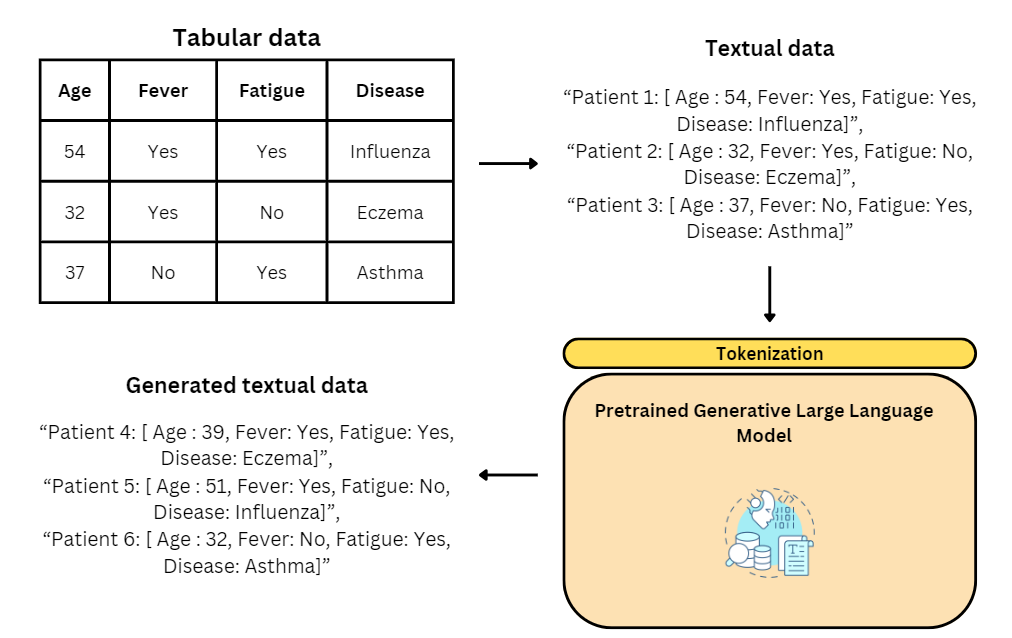
\includegraphics[width=0.85\textwidth]{images/pipeline.png}
    \caption{Data synthesis pipeline}
    \label{fig:pipeline}
\end{figure}

We propose a data synthesis pipeline consisting of several methodical steps. First, we propose to use two different datasets (small and large datasets) to evaluate the effectiveness of LLMs in generating data. This involves understanding how the data is going to be generated using LLMs. Then, a closer look is taken at the data to judge if it is essential to pre-process the data before using data synthesis methods. Next, state-of-the-art data generation models are leveraged to create high-fidelity synthetic data that closely resembles real-world information. Depending on the types of models utilized, they may give results in a different format than we initially wanted. In that case, post-processing is needed to convert the generated data into a CSV format. The CSV format will allow us to conduct a comparison and statistical analysis between the initial data and the generated one.

\section{Choices of Datasets}

In this paper, two datasets will be considered to ensure to validation of the results.
Given the ethical question around the manipulation of hospitals' data, the datasets used in this paper are publicly available and accessible via Kaggle.

\subsection{First Dataset}

The first dataset consists of 349 patients' health records in a CSV format (\cite{uom190346a_disease_symptoms_2021}). It contains 10 features including the patient's age, disease, and specific symptoms that are associated with the disease. 


This dataset quite is small given the number of patients. It will be used to generate the synthetic data, which is compared with the original data to perform statistical comparisons and also to train machine learning models to predict disease based on the other features.

It will be interesting to see how LLMs and GAN models can perform on such datasets.



\subsection{Second Dataset}

The second dataset consists of more than 4412 patients' health records (\cite{palivela_patient_treatment_2021}). It includes 11 features containing various haematological parameters measured in individuals, such as hematocrit, haemoglobin, erythrocyte count, leucocyte count, thrombocyte count, mean corpuscular haemoglobin (MCH), mean corpuscular haemoglobin concentration (MCHC), mean corpuscular volume (MCV), age, sex, and source of the sample (inpatient or outpatient). 

The second dataset is considered because the first dataset used is relatively small and might produce inaccurate generated results. Having a second dataset helps justify the results previously generated and it will be interesting to see how leveraging LLM power to provide relevant information based on such a large amount of information given initially.


\section{Choices of Models}

In our study, non-LLMs-based methods were utilized, more specifically, the model CTGAN (Conditional Tabular Generative Adversarial Network), inspired by Generative Adversarial Networks (GANs) adapted for data generation. The model is designed specifically for tabular data. Unlike other generative models that are often designed for image or text data, CTGAN is tailored to handle the unique challenges posed by tabular data, such as the presence of both continuous and categorical variables, and the need to maintain complex dependencies between columns (\cite{Xu2019}).


%A statistical model is used for data synthesis called Synthpop which is based on the R programming language.

%Both models mentioned above work directly with the CSV file being imported but with one particularity of being that Synthpop only works in R. 

%There is still a need, nonetheless, for pre-processing the data, more specifically, dealing with missing values, incoherent data formatting etc...

%%%%%%%%%%%%%%%%% CTGAN %%%%%%%%%%%%%%%%%%%%%%%%%%%%%%%%%%%%%%
\vspace{0.5cm}

\begin{figure}[ht!]
    \centering
    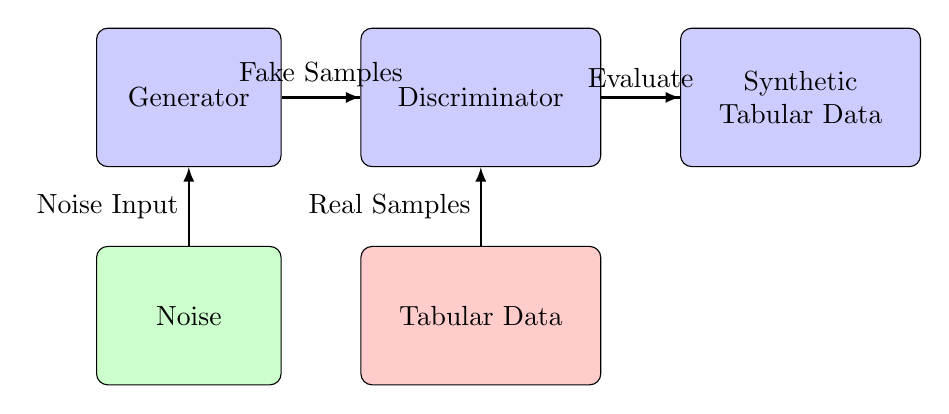
\begin{tikzpicture}[
        block/.style = {rectangle, draw, fill=blue!20, text width=6em, text centered, rounded corners, minimum height=5em},
        largerblock/.style = {rectangle, draw, fill=blue!20, text width=8em, text centered, rounded corners, minimum height=5em},
        line/.style = {draw, -latex, thick}, % Thicker lines and larger arrow tips
        textblock/.style = {text width=10em, text centered}
    ]
        % Nodes
        \node [block] (generator) {Generator};
        \node [largerblock, right=of generator, node distance=18cm] (discriminator) {Discriminator};
        \node [block, below=of generator, fill=green!20, node distance=8cm] (noise) {Noise};
        \node [largerblock, below=of discriminator, fill=red!20, node distance=8cm] (realdata) {Tabular Data};
        \node [largerblock, right=of discriminator, node distance=18cm] (output) {Synthetic Tabular Data};
        
        % Invisible nodes to extend arrows
        \node (gen_ext) [right=of generator, node distance=8cm] {};
        \node (disc_ext_left) [left=of discriminator, node distance=8cm] {};
        \node (disc_ext_right) [right=of discriminator, node distance=8cm] {};
        \node (out_ext) [left=of output, node distance=8cm] {};

        % Lines
        \path [line] (noise) -- (generator) node[midway, left] {Noise Input};
        \path [line] (generator.east) -- (gen_ext) -- (disc_ext_left) -- (discriminator.west) node[midway, above] {Fake Samples};
        \path [line] (realdata) -- (discriminator) node[midway, left] {Real Samples};
        \path [line] (discriminator.east) -- (disc_ext_right) -- (out_ext) -- (output.west) node[midway, above] {Evaluate};
    \end{tikzpicture}
    \caption{CTGAN Pipeline}
    \label{fig:gan_pipeline}
\end{figure}


CTGAN, just like GANs, is composed of two main components: a generator and a discriminator. They are trained simultaneously in a process where the generator tries to create synthetic data that is indistinguishable from real data, while the discriminator tries to distinguish between real and synthetic data.

\begin{itemize}
    \item[1.] \textsc{Generator}\\
    It takes random noise as input and generates synthetic data samples.

    \item[2.] \textsc{Discriminator}\\
    It evaluates the data samples and tries to classify them as real or synthetic. It provides feedback to the generator on how to improve the quality of the generated data.

    \item[3.] \textsc{Training} \\
    During training, the generator and discriminator are updated iteratively. The generator aims to minimize the probability of the discriminator correctly identifying the synthetic data, while the discriminator aims to maximize this probability. This adversarial training process continues until the discriminator can no longer distinguish between real and synthetic data effectively.
    
\end{itemize}


\vspace{1cm}

\noindent For the state-of-the-art LLMs, the following are the selected models:

\begin{itemize}
    \item[1.] \textsc{BeGreat model} \\
    The model is designed to generate synthetic data using LLMs. It specifically leverages the DistilGPT-2 model to fit and generate data. It is an open-source model, which makes it particularly suitable for creating anonymized data without compromising privacy (\cite{great_library_2024}).



    
    \item[2.] \textsc{LLaMa-3 model}, with 8 billion learning parameters.\\
    The open-source model, developed by Meta, is the state-of-the-art model for advanced text generation tasks. Available in two sizes 8 billion and 70 billion parameters, they are auto-regressive language models utilizing an optimized transformer architecture, which enhances their efficiency and scalability for various use cases (\cite{meta2024llama3, huggingface2024llama3}). Due to the computational limitations the model with 8 billion parameters.

    %\item Google's LLM called Gemma, 7 billion parameters version.
    %\item Mistral's LLM is called Mistral version 0.2 with 7 billion parameters.
\end{itemize}

\begin{figure}[H]
    \centering
    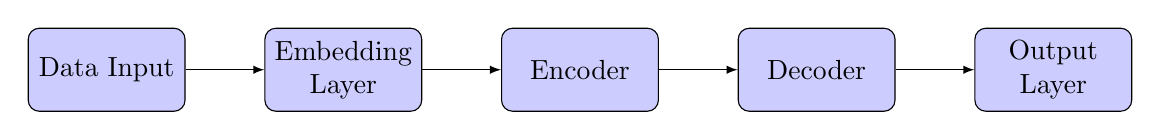
\begin{tikzpicture}[
        block/.style = {rectangle, draw, fill=blue!20, text width=5em, text centered, rounded corners, minimum height=3em},
        line/.style = {draw, -latex}, % Thicker lines and larger arrow tips
        node distance=1cm % Adjusted node distance for compactness
    ]
        % Nodes
        \node [block] (datainput) {Data Input};
        \node [block, right=of datainput] (embedding) {Embedding Layer};
        \node [block, right=of embedding] (encoder) {Encoder};
        \node [block, right=of encoder] (decoder) {Decoder};
        \node [block, right=of decoder] (output) {Output Layer};

        % Lines
        \draw [line] (datainput) -- (embedding);
        \draw [line] (embedding) -- (encoder);
        \draw [line] (encoder) -- (decoder);
        \draw [line] (decoder) -- (output);
    \end{tikzpicture}
    \caption{LLM Pipeline}
    \label{fig:llama3_pipeline}
\end{figure}

Such models require substantial computational resources; to address this, they are run on High-Performance Computation (HPC) clusters from the ADAPT Center. Nvidia's A100 GPUs 80GB within these clusters are utilized to run these state-of-the-art models efficiently.

Text-based prompts are the most prevalent approach for interacting with LLMs. More precisely, users provide a text prompt that explicitly describes what users want. They need to be clear enough so that LLMs can provide a high-quality and relevant response. Thus, more data pre-processing is necessary. As a matter of fact, the initial data is in tabular format which might infer with text prompts that the LLMs are receiving. We introduce thus, an additional data pre-processing that converts tabular data into textual data that we will go into detail later. 



\section{Data Pre-processing}

The data pre-processing encompasses a series of meticulous techniques aimed at transforming the initial dataset into a format that is interpretable by the data synthesis methods. This step plays a pivotal role as it ensures the quality and effectiveness of the data generation.

\vspace{0.5cm}
%%%%%%%%%%%%%%%%%%%%% INCONSISTENCIES %%%%%%%%%%%%%%%%%%%%%%%%

The initial data, when downloaded, might contain inconsistencies, errors, and missing values. The data cleaning process addresses these issues, which helps implement the data generative methods. In our cases, the process eliminates rows with missing information and fixes inconsistencies using the appropriate Python libraries.

\vspace{0.5cm}
%%%%%%%%%%%%%%%%%%% FURTHER LLMs %%%%%%%%%%%%%%%%%%%%%%%%%%%%%

Further data pre-processing is needed for the LLMs as the current data is in tabular format. A Python file class called TabularToTextualConverter is created, which includes a method called toTextual. It reads and converts each row and transforms it into a string containing all the features associated with that row. The associated features are separated by a comma which will help distinguish the different features for the LLMs. Thus, this method transforms tabular data into textual data. 

To illustrate the data pre-processing technique, consider the following dataset:

\begin{table}[H]
    \centering
    \renewcommand{\arraystretch}{1.5} % Increase cell height
    \setlength{\tabcolsep}{4pt} % Reduce column spacing
    \small % Reduce font size
    \begin{adjustbox}{max width=\textwidth}
    \begin{tabular}{|l|c|c|c|c|c|c|c|c|c|}
    \hline
    \makecell{\textbf{Disease}} & \makecell{\textbf{Fever}} & \makecell{\textbf{Cough}} & \makecell{\textbf{Fatigue}} & \makecell{\textbf{Difficulty} \\ \textbf{Breathing}} & \makecell{\textbf{Age}} & \makecell{\textbf{Gender}} & \makecell{\textbf{Blood} \\ \textbf{Pressure}} & \makecell{\textbf{Cholesterol} \\ \textbf{Level}} & \makecell{\textbf{Outcome} \\ \textbf{Variable}} \\ \hline
    Influenza & Yes & No & Yes & Yes & 19 & Female & Low & Normal & Positive \\ \hline
    \end{tabular}
    \end{adjustbox}
    \caption{Sample dataset with patient information}
    \label{table:sample_dataset}
\end{table}

After applying the data pre-processing steps described in our methodology, the transformed output for the first patient will be:

\begin{quote}
\textit{"Patient 1: [Disease: Influenza, Fever: Yes, Cough: No, Fatigue: Yes, Difficulty Breathing: Yes, Age: 19, Gender: Female, Blood Pressure: Low, Cholesterol Level: Normal, Outcome Variable: Positive]"}
\end{quote}

\vspace{0.5cm}

LLMs' input has a limit on the number of characters that they can accept. A method "getSubset" is created as a consequence, it subdivides the dataset into an equal number of subsets. 
Each request made for the LLM contains a subset of the dataset.

\begin{figure}[H]
    \centering
    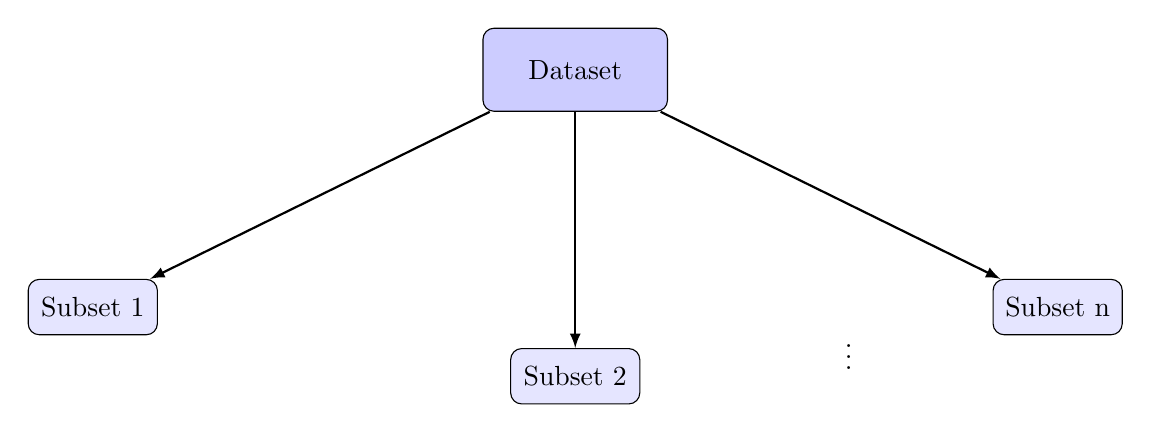
\begin{tikzpicture}[
        block/.style = {rectangle, draw, fill=blue!20, text width=6em, text centered, rounded corners, minimum height=3em},
        smallblock/.style = {rectangle, draw, fill=blue!10, text width=4em, text centered, rounded corners, minimum height=2em},
        line/.style = {draw, -latex, thick}, % Thicker lines and larger arrow tips
        node distance=3cm % Adjusted node distance for compactness
    ]
        % Nodes
        \node [block] (dataset) {Dataset};
        \node [smallblock, below left=of dataset, xshift=-2cm] (subset1) {Subset 1};
        \node [smallblock, below=of dataset] (subset2) {Subset 2};
        \node [smallblock, below right=of dataset, xshift=2cm] (subsetn) {Subset n};

        % Dots for continuation
        \node[below right=of dataset, yshift=-0.5cm] (dots) {$\vdots$};
        
        % Lines
        \draw [line] (dataset) -- (subset1);
        \draw [line] (dataset) -- (subset2);
        \draw [line] (dataset) -- (subsetn);
    \end{tikzpicture}
    \caption{Dataset Subdivision}
    \label{fig:dataset_subdivision}
\end{figure}

More details of the implementation can be found in the following appendix \ref{app:tabTotext_appendix}.


%\section{High-Performance Computing (HPC) setup}

%The HPC, as its name suggests, is designed to deliver cutting-edge computational power for tackling complex tasks such as the LLMs. It is composed of a network of interconnected servers equipped with advanced processors, graphics cards and storage. However, when I came to utilise it, I did not go as planned. In fact, some code that runs flawlessly on my personal computer fails to execute on the HPC infrastructure. The reason why certain codes failed to perform on the HPC infrastructure is that they utilise an older version of Linux, coupled with outdated libraries that are incompatible with the code I am employing. I have to go through a long process of updating the libraries. If you are wondering, I did not code directly on the HPC terminal, but I have used instead a remote SSH with Microsoft Vscode. I wanted to write this section of this paper because it took a very long time to figure out the issues and try to fix them. 





\section{Data Post-processing}

\begin{figure}[H]
    \centering
    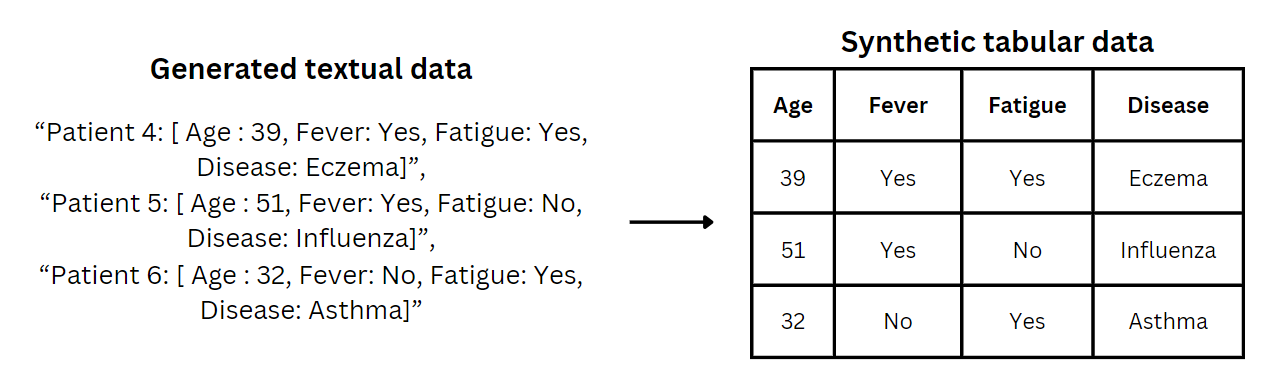
\includegraphics[width=0.85\textwidth]{images/textTotabular.png}
    \caption{Data synthesis pipeline}
    \label{fig:pipeline}
\end{figure}

The data post-processing deals with LLM responses which are stored in a TXT file. Unlike the data pre-processing, it also encompasses a series of meticulous techniques but, this time, it aims to transform the text file given by the LLMs into a CSV format file. The advantage of having a CSV file is to perform data analysis and compare it to the initial data. It will also help in comparing the models used and determining which is the one that performs the best. 

A Python class called TextualToTabularConverter is created, it is mainly based on regular expressions, to identify the matching patterns corresponding to the one that we specified in the text prompt given to the LLMs.
In cases where the regular expressions were not able to identify the patterns, because of the inconsistency of the LLMs' response, other pattern-matching methods are created specifically to identify the identify the exact pattern used by the LLMs.

More details of the implementation can be found in the following appendix \ref{app:textTotab_appendix}





% Define the specific LLM model and architecture to be used for data generation.

% Explain the data generation process, including data preparation, model training and evaluation

% Describe the metrics and evaluation criteria used to assess the quality adn realism of synthetic data.

% Discuss the potential biases and limitations of the chosen LLM model.






The evaluation of the results represents a critical part of the pipeline as it would determine if LLMs can provide performant results compared to GANs-based models.
However, it is important to select the right metrics to evaluate the data as they will be the ones that will judge if the data meets the quality standards and objectives of the analysis. The chosen metrics should align with the goals of the project and be capable of providing meaningful insights into the data's accuracy, relevance, and reliability.

\section{Evaluation}


As they are no official tools to measure how effective and safe is a synthetic data, there is, however, studies on how to empirically measure the effectiveness and the privacy. In this paper, we will be utilizing the state-of-the-art and complete Python framework called "Syntheval" to evaluate both the original and the synthetic data. %% ref to paper


\subsection{Measurement of the Similarity}

\begin{enumerate}
    \item Dimensionwise Means with 95\% of confidence intervals \\
    Scatter plots are utilized and the correlation confidence is measured to show how closely the synthetic data matches the values of the original data. 

    \item PCA Metrics \\
    The PCA eigenvalue difference is utilized to evaluate how well the synthetic data captures the variance and structure of the original data. A low value will indicate the model can capture the variance of the original data.

    \item Confidence Interval Overlap \\
    It measures how well the variability in the synthetic data matches the original data by comparing the overlap of their confidence intervals. A high value of the confidence interval overlap will show an inconsistency in preserving variability.

    \item Correlation Metrics \\
    The correlation matrix difference is calculated and it assesses how well the synthetic data preserves the relationships between variables in the original data. The smallest difference in correlation will show the best preservation of the relationships between the variables.

    \item Kolmogorov-Smirnov / Total Variation Distance Test \\
    The average combined statistics combine both Kolmogorov-Smirnov and Total Variation Distance Test values to evaluate the distributional similarity between synthetic and original data. A small average combined statistics will indicate the closest distributional match between the synthetic and original data.

    \item Empirical Hellinger Distance \\
    More precisely, the average Hellinger distance is calculated and it measures the similarity between probability distributions of the original and synthetic data. The smallest value of the average Hellinger distance will indicate the closest match to the original data’s distribution.

    \item Propensity Mean Squared Error (pMSE) \\
    pMSE evaluates how well the synthetic data mimics the original data for predictive modeling. A low value of the pMSE will show it effectively replicates the original data.

    \item Nearest Neighbour Adversarial Accuracy (NN Adversarial Accuracy)\\
    It assesses the distinguishability between synthetic and original data. A high value ensures the variability in distinguishability.

\end{enumerate}



\subsection{Measurement of the Accuracy of the Data}

In this section, the data and the synthetic data will be passed on to machine learning models to measure the accuracy. All models will be trained on the synthetic dataset and will be evaluated on the original dataset. The following machine learning models are utilized:

\begin{enumerate}
    \item Decision Tree Classifier \\
    A simple model, it can handle both numerical and categorical data.

    \item AdaBoost Classifier \\
    An improved version of the decision tree classifier focuses on the instances that are harder to classify and helps reduce the overall bias

    \item Random Forest Classifier \\
    The random forest classifier models are robust against overfitting as they leverage multiple decision trees.

    \item Logistic Regression \\
    Logistic regression is particularly effective for binary classification.
\end{enumerate}

\noindent Accuracy metrics are used to evaluate the generated data.

\begin{enumerate}
    \item Accuracy Real  (Acc R) \\
    It represents the classification accuracy of the original data. 

    \item Accuracy Fake (Acc F) \\
    It indicates the classification accuracy of the synthetic data.

    \item Absolute Difference ($|$Diff$|$) \\
    It shows the absolute difference between the accuracy real and the accuracy fake. This metric will show the discrepancy in the model's performance between the real and synthetic data.

    \item Error \\
    It represents the error rate of the model.
    
\end{enumerate}

\subsection{Measurement of the Data Privacy}


\begin{enumerate}
    \item Nearest Neighbour Distance Ratio \\
     It measures how close the synthetic data points are to the nearest real data points, with higher values indicating lower privacy.

    \item Median Distance to Closest Record \\
    measures the median distance from each synthetic data point to its nearest real data point, with higher values indicating better privacy.

    \item Hitting Rate (0.03 x Range(att)) \\
    It measures the fraction of synthetic data points that fall within a very small range of the real data points, with lower values indicating better privacy.

    \item Epsilon Identifiability Risk \\
    It measures the risk of re-identifying individuals in the synthetic data, with lower values indicating better privacy.

    \item Attribute Disclosure Risk (Accuracy) \\
    It measures the risk of accurately predicting sensitive attributes, with lower values indicating better privacy.
    
\end{enumerate}
\chapter{Implementation}
\lstset{language=Python, captionpos=b, frame=single}
\captionsetup{width=.8\linewidth} 


Guess what? At the beginning of each chapter, a description should introduce the reader to the content of the chapter. The description should explain to the reader the layout of the chapter, the contribution that the chapter makes to the overall dissertation and the contribution of the individual sections towards the overall chapter.


\section{Overview of the Solution}

%% Short caption for the table of listings - long caption for the explanation for the reader
\includecode{Sample Code}{Lengthy caption explaining the code to the reader}{lst:snippet}{snippet.py}

The code in listing~\ref{lst:snippet} is a demonstration how to include a file with code into the template.



\section{Component One}

%% Defaults for listings

The code in listing~\ref{lst:snippet2} is a demonstration how to include code in the template.

%% Short caption for the table of listings - long caption for the explanation for the reader
\begin{lstlisting}[caption={[Sample Code 2]Second Lengthy caption}, label={lst:snippet2}]
x = 1
if x == 1:
    # indented four spaces
    print("x is 1.")
\end{lstlisting}


\section{Summary}

Every chapter aside from the first and last chapter should conclude with a summary. 



\chapter{Results}
\label{ch:results}

% Present the results of data generation experiments, including visual inspection, statistical analysis, and correlation with real data.
\section{First Dataset}


\subsection{Statistical Distribution}

\subsubsection{Results}


The patient's age and disease will be studied, as the difference between the models is clearly illustrated.

\begin{figure}[H]
    \centering
    \begin{subfigure}[b]{0.45\textwidth}
        \centering
        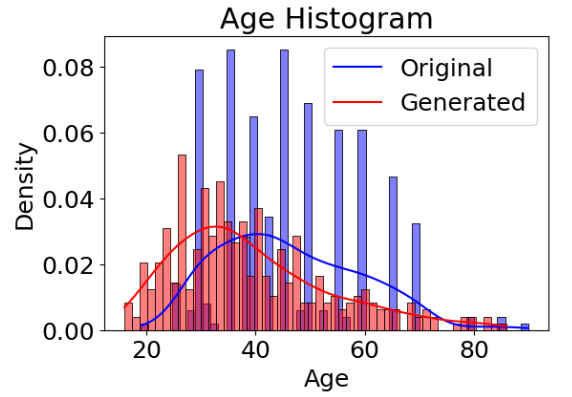
\includegraphics[width=\textwidth]{images/age_ctgan.png}
        \caption{CTGAN}
        \label{fig:age_ctgan}
    \end{subfigure}
    \hfill
    \begin{subfigure}[b]{0.45\textwidth}
        \centering
        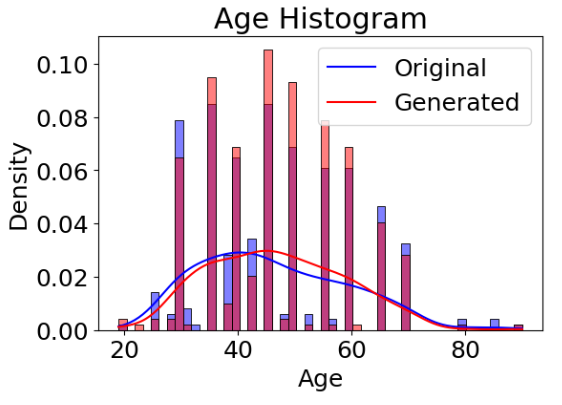
\includegraphics[width=\textwidth]{images/age_begreat.png}
        \caption{BeGreat}
        \label{fig:age_begreat}
    \end{subfigure}
    \hfill
    \begin{subfigure}[b]{0.45\textwidth}
        \centering
        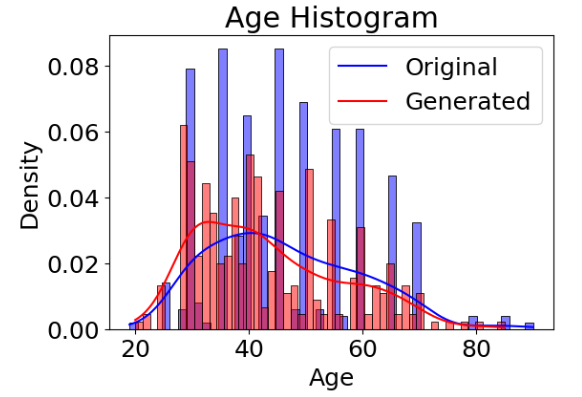
\includegraphics[width=\textwidth]{images/age_llama.png}
        \caption{LLaMa-3}
        \label{fig:age_llama}
    \end{subfigure}
    \caption{Age Distribution for Different Models}
    \label{fig:age_distrib}
\end{figure}

From figure \ref{fig:age_distrib}, the density curve \ref{fig:age_ctgan} shows that the CTGAN model can capture the dominant patient age demographic. Nonetheless, there is a slight variation compared to the original data.
The density curves, from \ref{fig:age_begreat}, indicate an almost perfect alignment between the generated data and the original data, showcasing the model's effectiveness in replicating the age distribution. The density curve from the LLaMa-3 model (\ref{fig:age_llama}) shows a very close alignment with the original data, but it is still better compared to the CTGAN and not as precise as the BeGreat model.


\begin{figure}[H]
    \centering
    \begin{subfigure}[b]{0.45\textwidth}
        \centering
        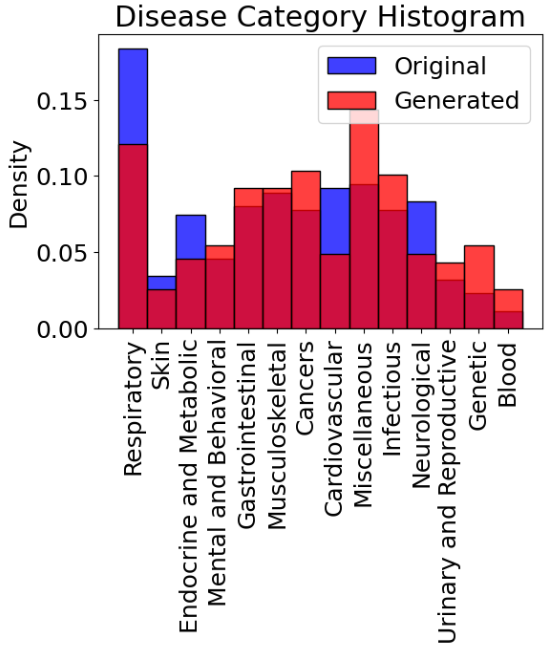
\includegraphics[width=\textwidth]{images/disease_ctgan.png}
        \caption{CTGAN}
        \label{fig:disease_ctgan}
    \end{subfigure}
    \hfill
    \begin{subfigure}[b]{0.45\textwidth}
        \centering
        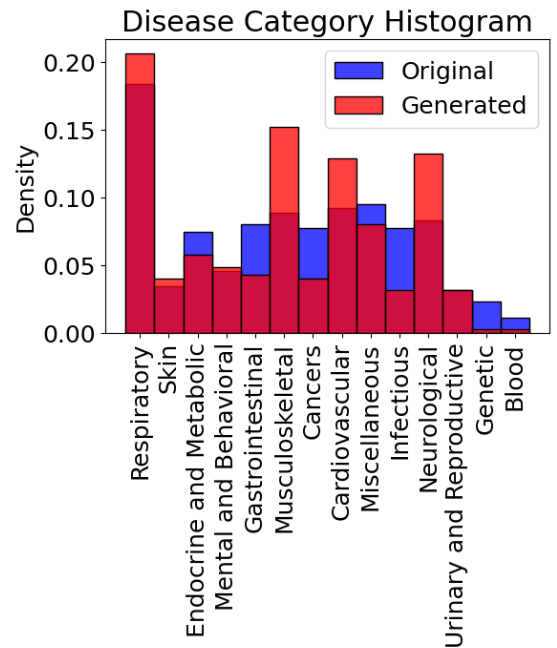
\includegraphics[width=\textwidth]{images/disease_begreat.png}
        \caption{BeGreat}
        \label{fig:disease_begreat}
    \end{subfigure}
    \hfill
    \begin{subfigure}[b]{0.45\textwidth}
        \centering
        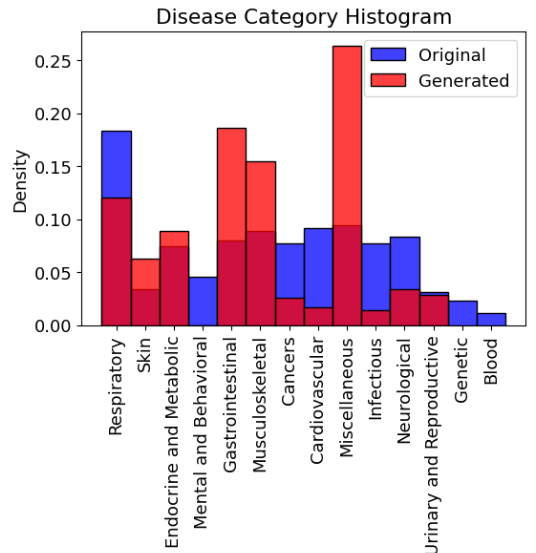
\includegraphics[width=\textwidth]{images/disease_llama.png}
        \caption{LLaMa-3}
        \label{fig:disease_llama}
    \end{subfigure}
    \caption{Comparison of Disease Categories Between Original and Generated Data for Different Models}
    \label{fig:disease_distrib}
\end{figure}

Figure \ref{fig:disease_distrib} illustrates the disease distribution from the original and synthetic data. CTGAN (\ref{fig:disease_ctgan}) as well as BeGreat (\ref{fig:disease_begreat}) replicate almost identical to the original data. However, LLaMa-3 (\ref{fig:disease_llama}) suggests a more different and diverse range of diseases with a high density for the miscellaneous category. LLaMa-3 was given a prompt where was asked the model to generate new diseases, which is why there is a higher density in the miscellaneous category.



%\begin{figure}[H]
%    \centering
%    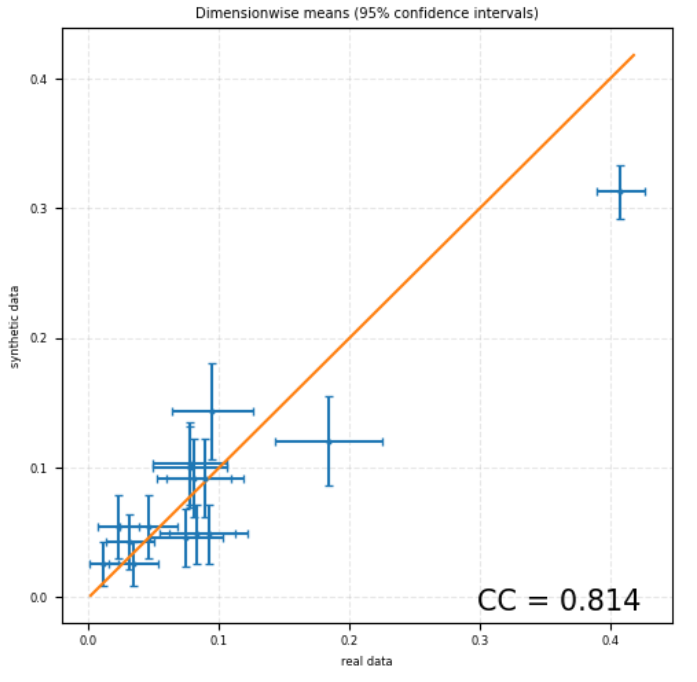
\includegraphics[width=1\linewidth]{images/avg_dim_ctgan.png}
%    \caption{Enter Caption}
%    \label{fig:enter-label}
%    \caption{Mutual Information Matrix Difference for Llama3 Model}
%    \label{fig:llama3_mutual_info}
%\end{figure}

\subsubsection{Summary}



\subsection{Comparative Analysis of Original and Synthetic Data}

\subsubsection{Results}


\begin{figure}[H]
    \centering
    \begin{subfigure}[b]{0.45\textwidth}
        \centering
        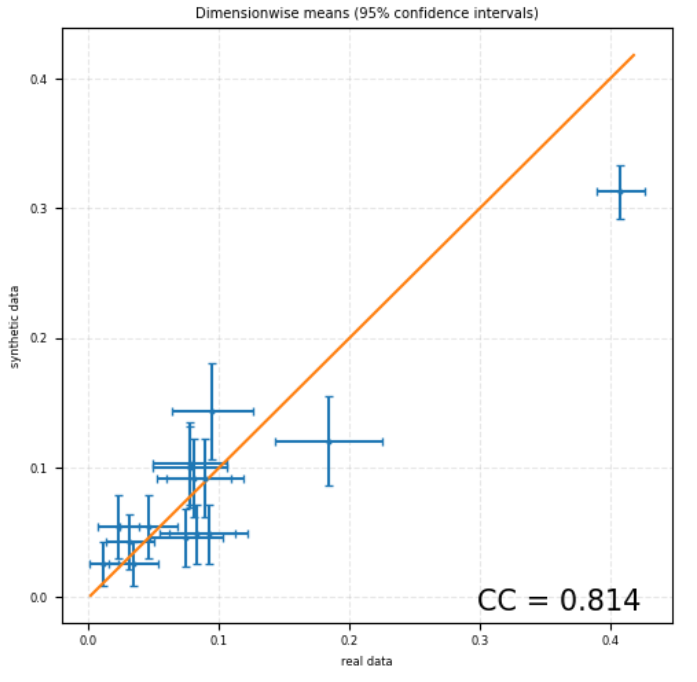
\includegraphics[width=\textwidth]{images/avg_dim_ctgan.png}
        \caption{CTGAN}
        \label{fig:avg_dim_ctgan}
    \end{subfigure}
    \hfill
    \begin{subfigure}[b]{0.45\textwidth}
        \centering
        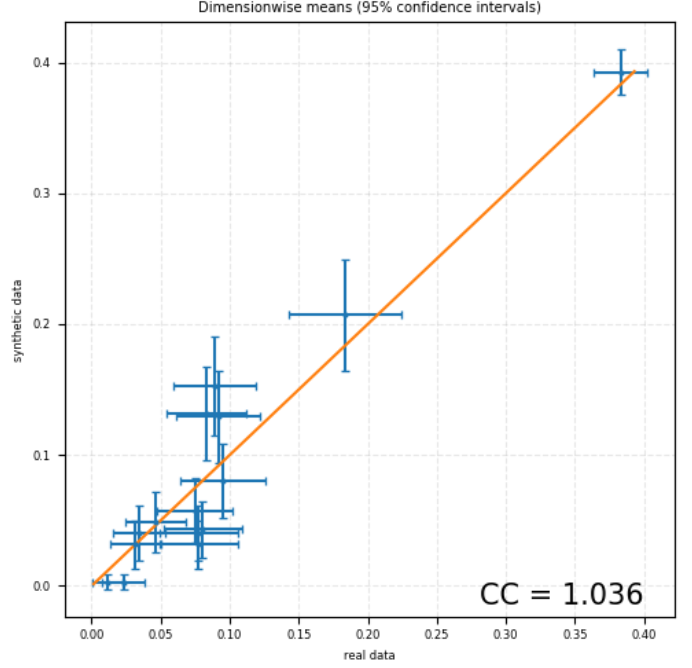
\includegraphics[width=\textwidth]{images/avg_dim_begreat.png}
        \caption{BeGreat}
        \label{fig:avg_dim_begreat}
    \end{subfigure}
    \hfill
    \begin{subfigure}[b]{0.48\textwidth}
        \centering
        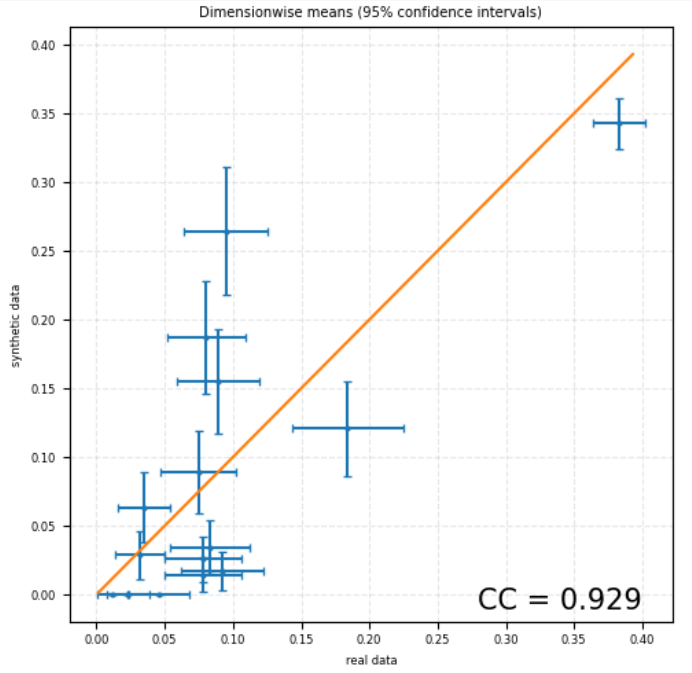
\includegraphics[width=\textwidth]{images/avg_dim_llama.png}
        \caption{LLaMa-3}
        \label{fig:avg_dim_llama}
    \end{subfigure}
    \caption{Dimensionwise means (95\% confidence intervals) scatter plots for different models}
    \label{fig:dim_means_distrib}
\end{figure}

Figure \ref{fig:dim_means_distrib} shows different scatter plots of the dimensionwise means with 95\% confidence intervals. The CTGAN model (\ref{fig:avg_dim_ctgan}) shows a correlation coefficient of 0.814, demonstrating that the model can synthesize correlated data to the original data with a high concentration of points in the lower values. However, the BeGreat model (\ref{fig:avg_dim_begreat}) has a correlation value of 1.036 which shows a perfect correlation between the synthetic and original data. This strong correlation can also be seen in the distribution \ref{fig:age_begreat}. LLaMa-3 has a correlation coefficient of 0.929 (\ref{fig:avg_dim_llama}), indicating that the model could capture the complex distribution of the original data.



\vspace{0.5cm}


\begin{figure}[H]
    \centering
        \centering
        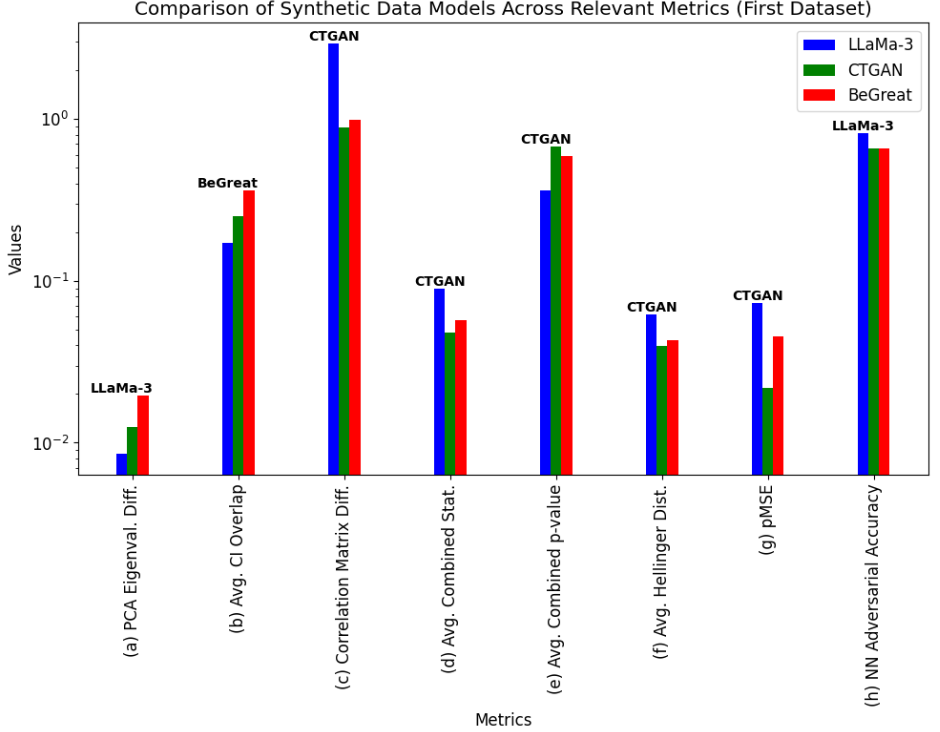
\includegraphics[width=1\textwidth]{images/dataset1_metrics.png}
        \caption{Comparison of synthetic data models across different metrics for the first dataset. In blue, LLaMa-3, in green CTGAN, in red BeGreat.}
        \label{fig:dataset1_metrics}
\end{figure}

\begin{enumerate}
    \item[(a)] PCA Eigenvalue Difference \\
    LLaMa-3 has the lowest PCA Eigenvalue Difference suggesting it best captures the variance of the original data. 

    \item[(b)] Average Confidence Interval Overlap \\
    BeGreat shows the highest average CI overlap indicating its consistency in preserving variability of the original data.

    \item[(c)] Correlation Matrix Difference \\
    CTGAN model preserves better the relationships between variables.

    \item[(d \& e)] Average Combined Statistics \& Average Combined p-value \\
    CTGAN model has the lowest value for the average combined statistics and the highest average combined p-value which both indicate the closest distributional match.

    \item[(f)] Average Hellinger Distance \\
    CTGAN model shows the lowest average Hellinger distance value indicating the closest match to the original data’s distribution.

    \item[(g)] pMSE \\
    CTGAN has low pMSE values, indicating it effectively replicates the original data.

    \item[(h)] NN Adversarial Accuracy \\
    Llama3 shows high adversarial accuracy, indicating variability in distinguishability.
\end{enumerate}

\subsubsection{Summary}

test


\subsection{Classification Accuracy Test Results}

The generated data consists of only 348 individual records, which is considered very low for training and evaluating machine learning models. A small training sample can lead to inaccuracies and biased outcomes. 


\begin{figure}[H]
    \centering
        \centering
        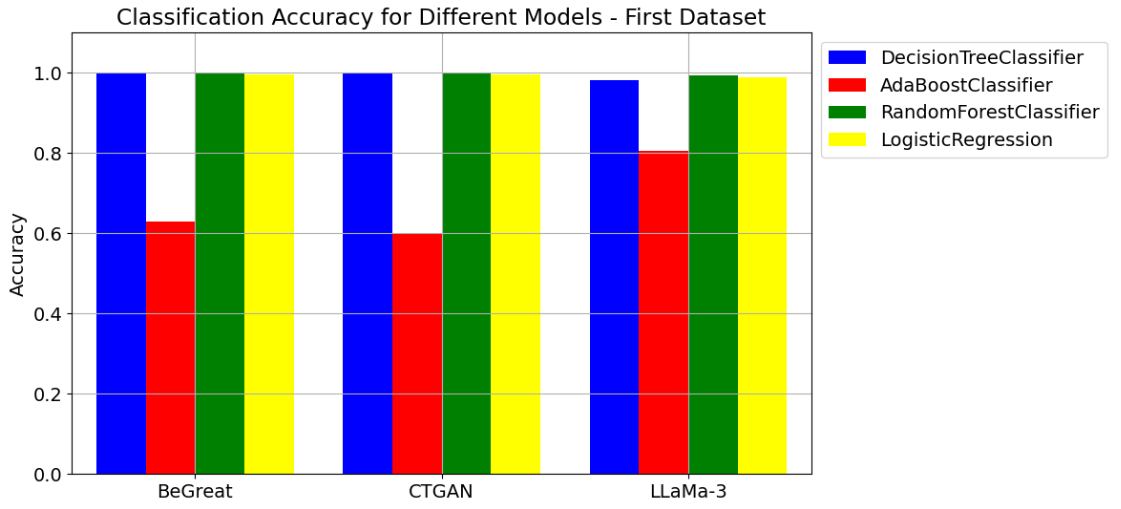
\includegraphics[width=1\textwidth]{images/dataset1_ml.png}
        \caption{Comparison of classification accuracy across machine learning models for the first dataset using Decision Tree Classifier, AdaBoost Classifier, Random Forest Classifier, and Logistic Regression.}
        \label{fig:dataset1_ml}
\end{figure}

Figure \ref{fig:dataset1_ml} shows the performance of different machine learning models using the first dataset. The decision tree, random forest classifiers and the logistic regression all show high accuracies. This is highly due to the fact that the model has been trained on a small sample and cannot give consistent and accurate results. However, the AdaBoost classifier was able to capture the difference lying in the different generated data. LLaMa-3 is outperforming both BeGreat and CTGAN and demonstrates the highest overall accuracies. The same goes for the BeGreat model it was able to perform better than CTGAN.



\subsection{Privacy Metrics Comparison}

For better visualization, the results of the data privacy metrics are normalized. 


\begin{figure}[H]
    \centering
        \centering
        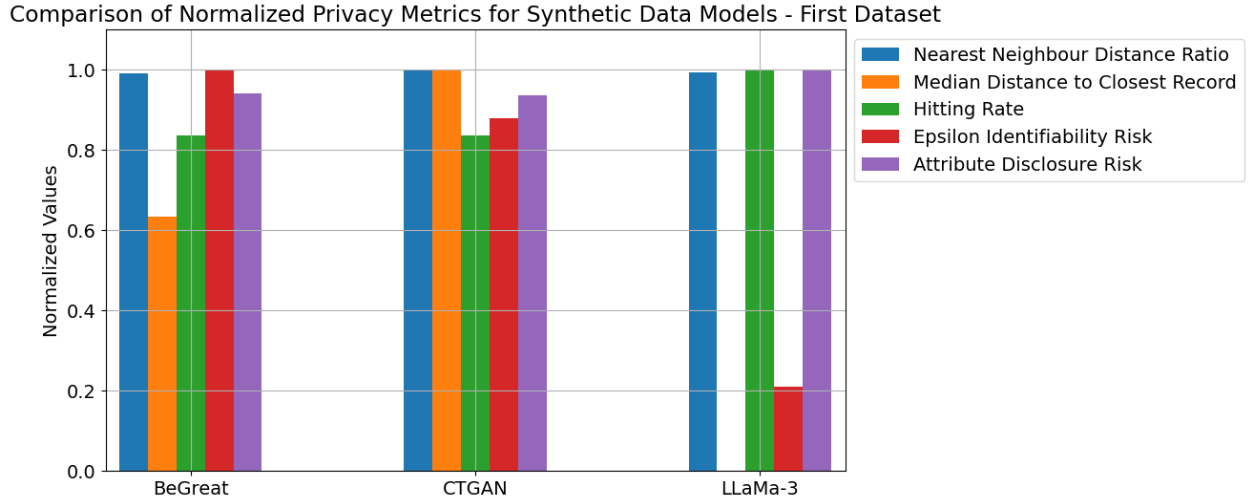
\includegraphics[width=1\textwidth]{images/dataset1_privacy.png}
        \caption{Comparison of normalised privacy metrics for synthetic data models in the first dataset.}
        \label{fig:dataset1_privacy}
\end{figure}

Figure \ref{fig:dataset1_privacy} shows various privacy metrics results of the different models.

\begin{enumerate}
    \item[(a)] Nearest Neighbour Distance Ratio \\
    All models show very close values to 1.0. However, a high value of the neatest neighbour distance ratio indicates a low privacy. Digging into the precise values of the metric, which can be found in the appendix, the BeGreat suggests a lower value compared to the other two models. Nonetheless, data privacy is not respected for all models for that particular metric.

    \item[(b)] Median Distance to Closest Record \\
    CTGAN shows the highest median distance to the closest record, indicating the best privacy. Model BeGreat follows after the CTGAN model, while Model Llama3 has an infinite median distance, suggesting perfect privacy. % need to be checked

    
    \item[(c)] Hitting Rate \\
    LLaMa-3 suggests a higher hitting rate (0.0172), indicating slightly low privacy. BeGreat and CTGAN show the lowest hitting rate (0.0144), indicating better privacy. However, all hitting rates are close to the value 0 which in that case the normalization is not suited for this metric. Thus, all models contribute to better data privacy.


    \item[(d)] Epsilon Identifiability Risk \\
    LLaMa-3 shows the lowest epsilon identifiability risk (0.0805), followed by CTGAN (0.3381). BeGreat has the highest risk (0.3849). CTGAN and BeGreat have almost the same risk value, which suggests lower privacy. On the other hand, LLaMa-3 has a value much closer to 0, indicating that it performs better at generating data with a low risk of exposing real information. 

    \item[(e)] Attribute Disclosure Risk \\
    CTGAN shows the lowest attribute disclosure risk (0.7993), followed closely by BeGreat (0.8044). Llama3 has the highest risk (0.8540), indicating lower privacy. However, all models have a relatively high value of the attribute disclosure risk, which suggests they are as vulnerable as the others. %% better reformulation
    
\end{enumerate}




%%%%%%%%%%%%%%%%%%%%%%%%%%%%%%%%%%%%%%%%%%%%%%%%%%%%%%%%%%%%%%%%%%%%%%%%%%%%%%%%%%%%%%%%%%%%%%%%%%%%%%%%%%%%%%%%%%%%%%%%%%%%%%%%%%%%%%%%%%%%%%%%%%%%%%%%%%%%%%%%%%%%%%%%%%%%%%%%%%%%%%%%%%%%%%%%%%%%%%%%%%%%%%%%%%%%%%%%%%%%%%%%%%%%%%%%%%%%%%%%%%%%%%%%%%%%%%%%%%%%%%%%%%%%%%%%%%%%%%%%%%%%%%%%%%%%%%%%%%%%%%%%%%%%%%%%%%%%%%%%%%%%%%%%%%%%%%%%%%%%%%%%%%%%%%%%%%%%%%%%%%%%%%%%%%%%%%%%%%%%%%%%%%%%%%%%%%%%%%%%%%%%%%%%%%%%%%%%%%%%%%%%%%%%%%%%%%%%%%%%%%%%%%%%%%%%%%%%%%%%



\section{Second Dataset}

\subsection{Statistical Distribution}

\subsection{Comparative Analysis of Original and Synthetic Data}

\begin{figure}[H]
    \centering
    \begin{subfigure}[b]{0.47\textwidth}
        \centering
        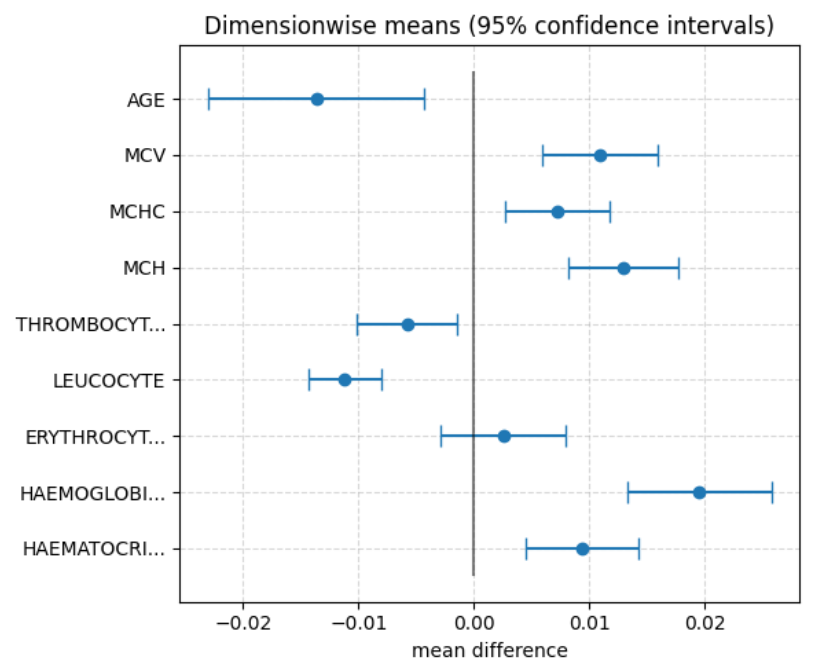
\includegraphics[width=\textwidth]{images/avg_dim_2_ctgan.png}
        \caption{CTGAN}
        \label{fig:avg_dim_2_ctgan}
    \end{subfigure}
    \hfill
    \begin{subfigure}[b]{0.47\textwidth}
        \centering
        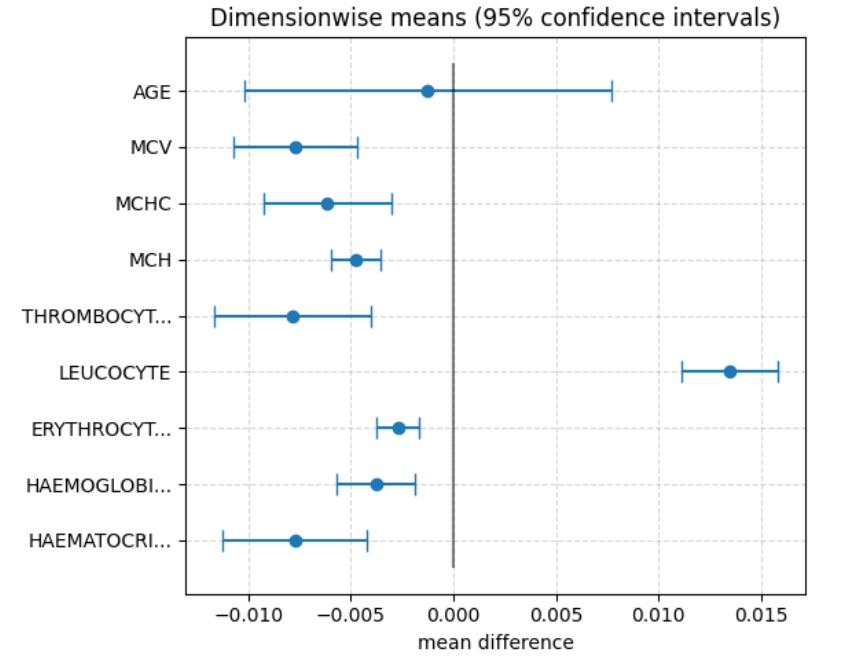
\includegraphics[width=\textwidth]{images/avg_dim_2_begreat.png}
        \caption{BeGreat}
        \label{fig:avg_dim_2_begreat}
    \end{subfigure}
    \hfill
    \begin{subfigure}[b]{0.48\textwidth}
        \centering
        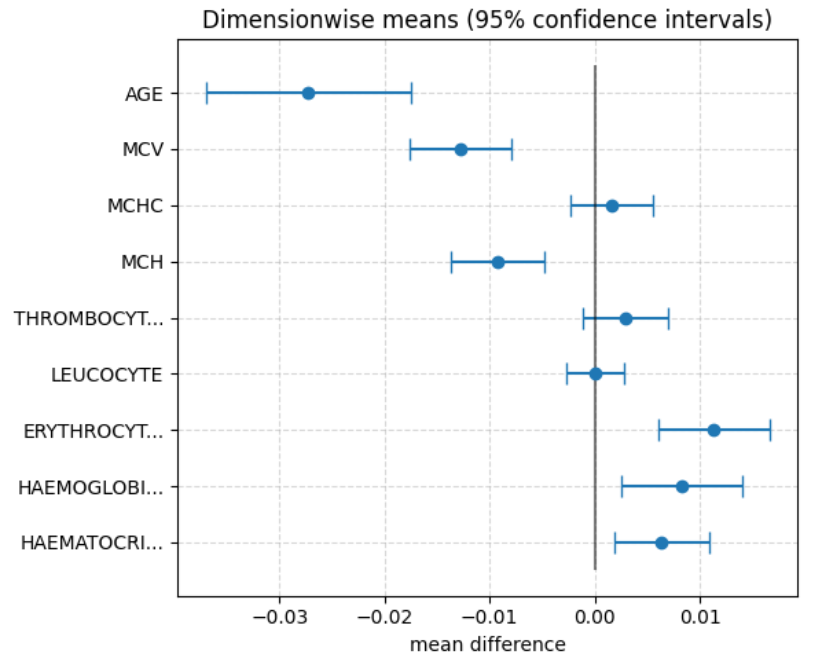
\includegraphics[width=\textwidth]{images/avg_dim_2_llama.png}
        \caption{LLaMa-3}
        \label{fig:avg_dim_2_llama}
    \end{subfigure}
    \caption{Dimensionwise means (95\% confidence intervals) mean-difference plot for different models}
    \label{fig:dim_means_distrib_2}
\end{figure}


Figure \ref{fig:dim_means_distrib_2} shows the mean-difference plots for different models. LLaMa-3 (\ref{fig:avg_dim_2_llama}) shows a drastic shift of the 'AGE' from the zero difference line (black vertical bar) showing that the model tends to generate more variability for the patient's age compared with the original data. On the other hand, the BeGreat model (\ref{fig:avg_dim_2_begreat}) shows a much closer 'AGE' variability from the original data. 
The BeGreat model shows relatively close values from the zero difference line for the other variables indicating that these variables are closer to the real data's variables. Conversely, the CTGAN and the LLaMa-3 model both depict more varied mean differences of variables such as MCV, ERYTHROCYTE etc... leading to more distinct data than the original data. 




\begin{figure}[H]
    \centering
        \centering
        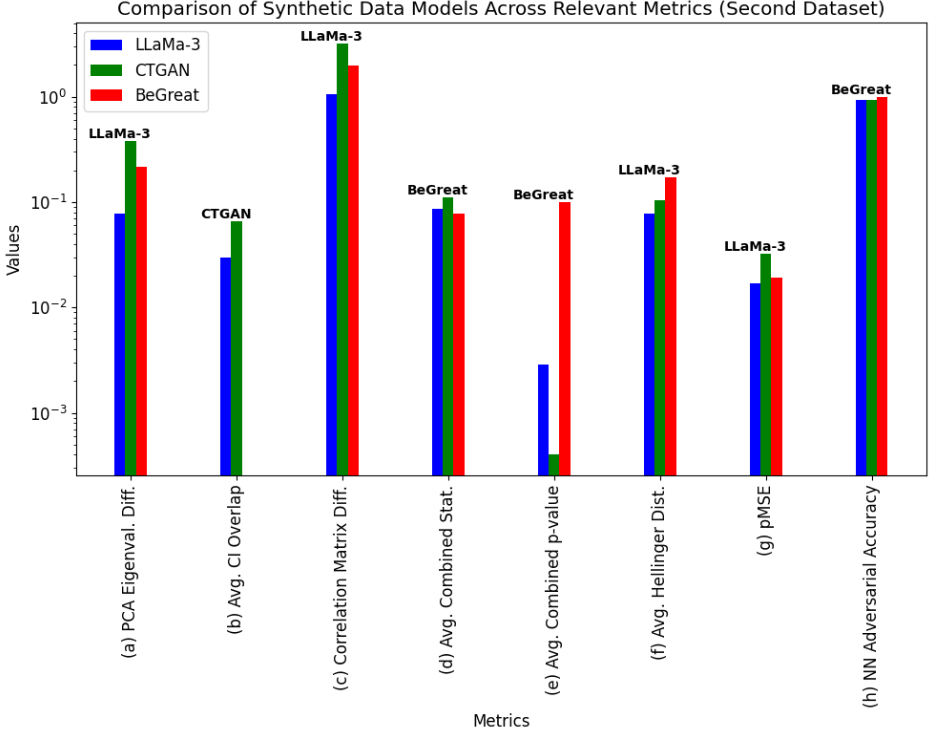
\includegraphics[width=1\textwidth]{images/dataset2_metrics.png}
        \caption{Comparison of synthetic data models across different metrics for the second dataset. In blue, LLaMa-3, in green CTGAN, in red BeGreat.}
        \label{fig:dataset2_metrics}
\end{figure}

\begin{enumerate}
    \item[(a)] PCA Eigenvalue Difference \\
    LLaMa-3 has the lowest PCA Eigenvalue Difference suggesting it best captures the variance of the original data. 

    \item[(b)] Average Confidence Interval Overlap \\
    CTGAN shows the highest average CI overlap indicating its consistency in preserving variability of the original data.

    \item[(c)] Correlation Matrix Difference \\
    LLaMa-3 model preserves better the relationships between variables.

    \item[(d \& e)] Average Combined Statistics \& Average Combined p-value \\
    BeGreat model has the lowest value for the average combined statistics and the highest average combined p-value which both indicate the closest distributional match.

    \item[(f)] Average Hellinger Distance \\
    LLaMa-3 model shows the lowest average Hellinger distance value indicating the closest match to the original data’s distribution.

    \item[(g)] pMSE \\
    LLaMa-3 has low pMSE values, indicating it effectively replicates the original data.

    \item[(h)] NN Adversarial Accuracy \\
    BeGreat shows high adversarial accuracy, indicating variability in distinguishability.
\end{enumerate}

\subsubsection{Summary}

test



\subsection{Classification Accuracy Test Results}




\begin{figure}[H]
    \centering
        \centering
        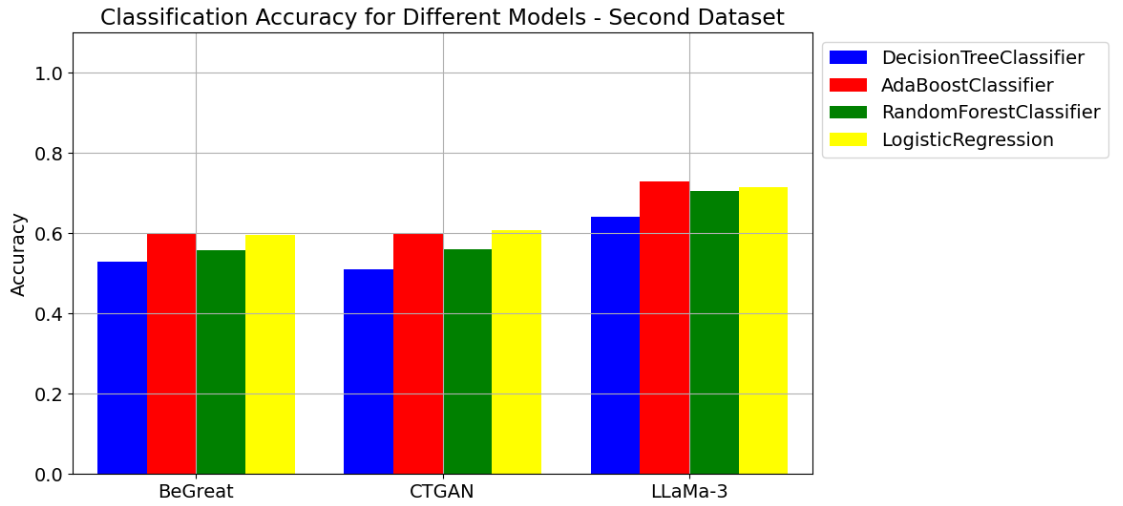
\includegraphics[width=1\textwidth]{images/dataset2_ml.png}
        \caption{Comparison of classification accuracy across machine learning models for the second dataset using Decision Tree Classifier, AdaBoost Classifier, Random Forest Classifier, and Logistic Regression.}
        \label{fig:dataset2_ml}
\end{figure}

Figure \ref{fig:dataset2_ml} shows the performance results of the different machine learning models. It can be observed that CTGAN and the BeGreat model have similar accuracy results. However, the LLaMa-3 model outperforms both the BeGreat and CTGAN models across all machine learning models.





\subsection{Privacy Metrics Comparison}

\begin{figure}[H]
    \centering
        \centering
        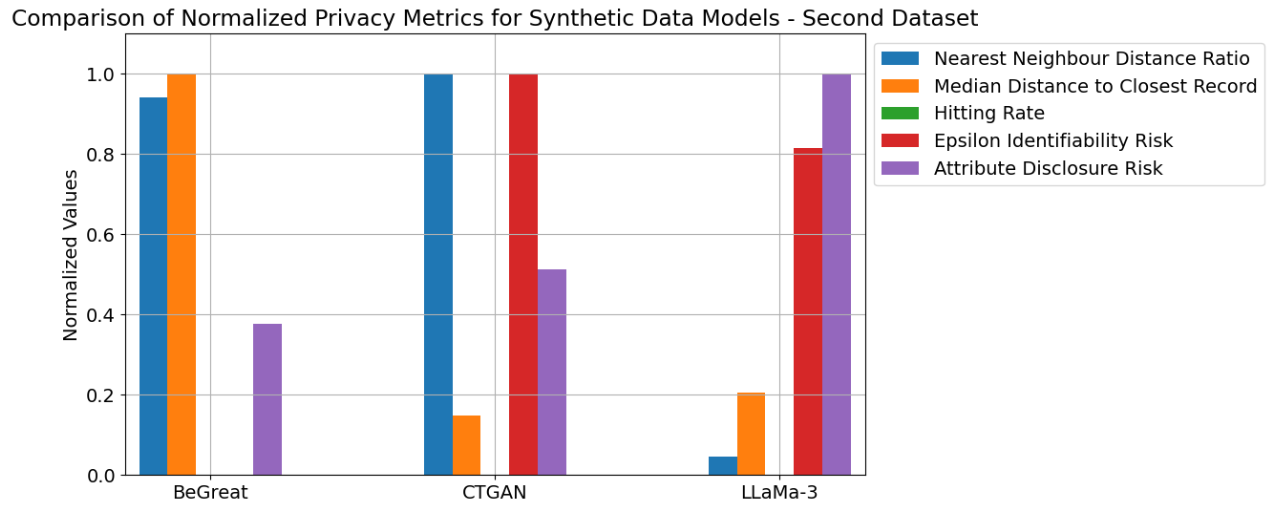
\includegraphics[width=1\textwidth]{images/dataset2_privacy.png}
        \caption{Comparison of normalised privacy metrics for synthetic data models in the second dataset.}
        \label{fig:dataset2_privacy}
\end{figure}


\begin{enumerate}
    \item[(a)] Nearest Neighbour Distance Ratio \\
    The CTGAN model exhibits the highest value among the other models, this suggests a closer generated data to the real data which tends to lower the privacy. On the other hand, the LLaMa-3 model shows a much lower value for this metric suggesting better privacy preservation in terms of distance from real data.

    \item[(b)] Median Distance to Closest Record \\
    CTGAN shows the lowest median distance to the closest record, indicating that the synthetic data is very close to the real data, which might raise privacy concerns. However, both BeGreat and LLaMa-3 have higher values suggesting perfect privacy.

    
    \item[(c)] Hitting Rate \\
    However, all hitting rates are close to the value 0 which indicates that all models contribute to better privacy.


    \item[(d)] Epsilon Identifiability Risk \\
    BeGreat shows the lowest epsilon identifiability risk (0.0002), followed by LLaMa-3 (0.1729). CTGAN has the highest risk (0.2122). CTGAN and LLaMa-3 have around the same risk value, which suggests lower privacy. On the other hand, BeGreat has a value much closer to 0, indicating that it performs better at generating data with a low risk of exposing real information. 

    \item[(e)] Attribute Disclosure Risk \\
    BeGreat shows the lowest attribute disclosure risk, followed closely by CTGAN. LLaMa-3 has the highest risk, indicating lower privacy. However, all models have a relatively high value of the attribute disclosure risk, which suggests they are as vulnerable as the others. %% better reformulation
    
\end{enumerate}















\vspace{10cm}




\section{Comparative Analysis of Original and Synthetic Data}

\subsection{Average Dimensionwise Means Difference}

\begin{table}[H]
\centering
\caption{Average Dimensionwise Means Difference for Synthetic Data Models}
\label{tab:avg_means_diff_combined}
\begin{tabularx}{\textwidth}{l*{6}{X}}
    \toprule
    \textbf{Model} & \multicolumn{3}{c}{\textbf{First Data}} & \multicolumn{3}{c}{\textbf{Second Data}} \\
    \cmidrule(lr){2-4} \cmidrule(lr){5-7}
    & \textbf{Llama3} & \textbf{CTGAN} & \textbf{BeGreat} & \textbf{Llama3} & \textbf{CTGAN} & \textbf{BeGreat} \\
    \midrule
    Avg. Means Diff. & 0.0586 ± 0.0062 & 0.0281 ± 0.0052 & 0.0325 ± 0.0051 & 0.0266 ± 0.0009 & 0.0232 ± 0.0010 & 0.0170 ± 0.0007 \\
    \bottomrule
\end{tabularx}
\end{table}



From Table \ref{tab:avg_means_diff_combined}, we can analyze the performance of each model across both data sets:

\textbf{BeGreat} has the smallest mean difference in both data sets, indicating it most accurately replicates the average values of the original data.
\textbf{CTGAN} follows closely, showing slightly higher average means differences but still demonstrating good accuracy.
\textbf{Llama3} has the largest mean difference in both data sets but still maintains a reasonable level of accuracy.

\vspace{0.5cm}


The comparison of average dimensionwise means differences reveals that:

\textbf{BeGreat} consistently provides the best performance in terms of replicating the original data's mean values across both data sets.
\textbf{CTGAN} also performs well, showing small differences in average means but slightly larger than BeGreat.
\textbf{Llama3} shows the largest differences but remains within an acceptable range of accuracy.


\vspace{0.5cm}

These findings highlight the strengths of each model in replicating the original data's mean values. The BeGreat model is recommended for applications requiring the highest fidelity in replicating mean values, while the CTGAN model offers a balanced performance. The Llama3 model, although showing slightly larger differences, still provides reasonable accuracy and may be suitable for applications with less stringent requirements on mean value replication.




\subsection{PCA Metrics}

\begin{table}[H]
\centering
\caption{PCA Metrics for Synthetic Data Models}
\label{tab:pca_metrics_combined}
\begin{tabularx}{\textwidth}{l*{6}{X}}
    \toprule
    \textbf{Metric Description} & \multicolumn{3}{c}{\textbf{First Data}} & \multicolumn{3}{c}{\textbf{Second Data}} \\
    \cmidrule(lr){2-4} \cmidrule(lr){5-7}
    & \textbf{Llama3} & \textbf{CTGAN} & \textbf{BeGreat} & \textbf{Llama3} & \textbf{CTGAN} & \textbf{BeGreat} \\
    \midrule
    PCA Eigenval. Diff. & 0.0085 & 0.0125 & 0.0196 & 0.0781 & 0.3825 & 0.2181 \\
    PCA Eigenvec. Angle & 1.0226 & 0.9035 & 1.5565 & 0.9489 & 1.5186 & 0.2738 \\
    \bottomrule
\end{tabularx}
\end{table}


From Table \ref{tab:pca_metrics_combined}, the PCA metrics evaluate how well the synthetic data captures the variance and structure of the original data:

\textbf{Llama3} consistently shows the smallest eigenvalue difference in both datasets, indicating it best captures the variance of the original data.
\textbf{BeGreat} excels in preserving the structural similarity in the second dataset but not as well in the first dataset.
\textbf{CTGAN} shows the largest differences in both metrics in the second dataset but performs better in the first dataset, particularly in preserving structural similarity.

\vspace{0.5cm}

The comparison of PCA metrics reveals that:

\textbf{Llama3} consistently provides the best performance in terms of capturing the variance of the original data across both datasets.
\textbf{BeGreat} shows a strong performance in preserving structural similarity in the second dataset but less so in the first dataset.
\textbf{CTGAN} performs well in the first dataset but shows larger differences in the second dataset, indicating variability in its effectiveness.

\vspace{0.5cm}

These findings highlight the strengths and limitations of each model in terms of PCA metrics. The Llama3 model is recommended for applications requiring high fidelity in capturing the variance of the original data, while the BeGreat model offers strong performance in preserving structural similarity in certain cases. The CTGAN model, while showing good performance in some cases, may require further refinement for consistent results.








\subsection{Confidence Interval Overlap}

\begin{table}[H]
\centering
\caption{Confidence Interval Overlap for Synthetic Data Models}
\label{tab:ci_overlap_combined}
\begin{tabularx}{\textwidth}{l*{6}{X}}
    \toprule
    \textbf{Metric Description} & \multicolumn{3}{c}{\textbf{First Data}} & \multicolumn{3}{c}{\textbf{Second Data}} \\
    \cmidrule(lr){2-4} \cmidrule(lr){5-7}
    & \textbf{Llama3} & \textbf{CTGAN} & \textbf{BeGreat} & \textbf{Llama3} & \textbf{CTGAN} & \textbf{BeGreat} \\
    \midrule
    Avg. CI Overlap & 0.1725 ± 0.1038 & 0.2497 ± 0.0805 & 0.3632 ± 0.0996 & 0.0300 ± 0.0300 & 0.0654 ± 0.0437 & 0.0000 ± 0.0000 \\
    \# Non-overlapping CIs & 9 & 7 & 7 & 8 & 7 & 9 \\
    Frac. Non-overlapping CIs & 0.7500 & 0.4667 & 0.4667 & 0.8889 & 0.7778 & 1.0000 \\
    \bottomrule
\end{tabularx}
\end{table}



From Table \ref{tab:ci_overlap_combined}, the confidence interval overlap measures how well the variability in the synthetic data matches the original data:

\textbf{BeGreat} shows no overlap in the second dataset but the highest average CI overlap in the first dataset, indicating inconsistency in preserving variability.
\textbf{CTGAN} performs well in both datasets, showing the highest average CI overlap in the second dataset and a strong performance in the first dataset.
\textbf{Llama3} shows moderate performance in both datasets, with lower average CI overlap compared to CTGAN and BeGreat.

\vspace{0.5cm}

The comparison of confidence interval overlap reveals that:

\textbf{CTGAN} consistently provides good performance in terms of preserving variability across both datasets.
\textbf{BeGreat} shows strong performance in the first dataset but no overlap in the second dataset, indicating variability in its effectiveness.
\textbf{Llama3} shows moderate performance in both datasets but generally lower average CI overlap compared to CTGAN and BeGreat.

\vspace{0.5cm}

These findings highlight the strengths and limitations of each model in terms of confidence interval overlap. The CTGAN model is recommended for applications requiring consistent preservation of variability, while the BeGreat model offers strong performance in some cases. Although the Llama3 model shows moderate performance, it may be suitable for applications with less stringent requirements for variability preservation.





\subsection{Correlation Metrics}

\begin{table}[H]
\centering
\caption{Correlation Metrics for Synthetic Data Models}
\label{tab:correlation_metrics_combined}
\begin{tabularx}{\textwidth}{l*{6}{X}}
    \toprule
    \textbf{Metric Description} & \multicolumn{3}{c}{\textbf{First Data}} & \multicolumn{3}{c}{\textbf{Second Data}} \\
    \cmidrule(lr){2-4} \cmidrule(lr){5-7}
    & \textbf{Llama3} & \textbf{CTGAN} & \textbf{BeGreat} & \textbf{Llama3} & \textbf{CTGAN} & \textbf{BeGreat} \\
    \midrule
    Correlation Matrix Diff. & 2.9316 & 0.8911 & 0.9849 & 1.0608 & 3.2077 & 1.9991 \\
    Mutual Info. Diff. & 2.7911 & 0.6086 & 0.5918 & 0.1937 & 0.2485 & 1.1123 \\
    \bottomrule
\end{tabularx}
\end{table}




From Table \ref{tab:correlation_metrics_combined}, correlation metrics assess the preservation of relationships between variables:

\textbf{Llama3} consistently shows the smallest differences in both correlation metrics across both datasets, indicating it best preserves the relationships between variables.
\textbf{CTGAN} shows larger differences in the second dataset but performs reasonably well in the first dataset.
\textbf{BeGreat} has the largest differences in mutual information in the second dataset and a missing value for the correlation matrix difference in the first dataset, indicating variability in its effectiveness.

\vspace{0.5cm}

The comparison of correlation metrics reveals that:

\textbf{Llama3} consistently provides the best performance in terms of preserving relationships between variables across both datasets.
\textbf{CTGAN} performs well in the first dataset but shows larger differences in the second dataset, indicating variability in its effectiveness.
\textbf{BeGreat} shows the largest differences in mutual information in the second dataset and has inconsistent results in the first dataset.

\vspace{0.5cm}

These findings highlight the strengths and limitations of each model in terms of correlation metrics. The Llama3 model is recommended for applications requiring high fidelity in preserving relationships between variables, while the CTGAN model offers reasonable performance in some cases. The BeGreat model, although showing some inconsistencies, may still be suitable for certain applications with less stringent requirements on preserving relationships.








\subsection{Kolmogorov-Smirnov / Total Variation Distance Test}



\begin{table}[H]
\centering
\caption{Kolmogorov-Smirnov / Total Variation Distance Test for Synthetic Data Models}
\label{tab:ks_tv_test_combined}
\begin{tabularx}{\textwidth}{l*{6}{X}}
    \toprule
    \textbf{Metric Description} & \multicolumn{3}{c}{\textbf{First Data}} & \multicolumn{3}{c}{\textbf{Second Data}} \\
    \cmidrule(lr){2-4} \cmidrule(lr){5-7}
    & \textbf{Llama3} & \textbf{CTGAN} & \textbf{BeGreat} & \textbf{Llama3} & \textbf{CTGAN} & \textbf{BeGreat} \\
    \midrule
    Avg. Combined Stat. & 0.0894 ± 0.0185 & 0.0478 ± 0.0120 & 0.0573 ± 0.0118 & 0.0863 ± 0.0174 & 0.1110 ± 0.0201 & 0.0781 ± 0.0140 \\
    Avg. KS Dist. & 0.0699 ± 0.0167 & 0.0426 ± 0.0159 & 0.0400 ± 0.0126 & 0.0974 ± 0.0193 & 0.0946 ± 0.0196 & 0.0936 ± 0.0117 \\
    Avg. TV Dist. & 0.1089 ± 0.0330 & 0.0565 ± 0.0186 & 0.0860 ± 0.0207 & 0.0362 ± 0.0121 & 0.1848 ± 0.0404 & 0.0087 ± 0.0080 \\
    Avg. Combined p-value & 0.3600 ± 0.0858 & 0.6765 ± 0.0812 & 0.5865 ± 0.0850 & 0.0029 ± 0.0027 & 0.0004 ± 0.0003 & 0.1006 ± 0.0887 \\
    \# Sig. Tests (\(\alpha=0.05\)) & 9 & 2 & 6 & 11 & 11 & 9 \\
    Frac. Sig. Tests & 0.3750 & 0.0833 & 0.2500 & 1.0000 & 1.0000 & 0.8182 \\
    \bottomrule
\end{tabularx}
\end{table}



From Table \ref{tab:ks_tv_test_combined}, the Kolmogorov-Smirnov (KS) and Total Variation (TV) distance tests evaluate the distributional similarity between synthetic and original data:

\textbf{BeGreat} consistently shows the smallest combined statistics and high p-values across both datasets, indicating the closest distributional match.
\textbf{Llama3} performs well, with moderate combined statistics and reasonable p-values, indicating a good distributional match.
\textbf{CTGAN} shows larger combined statistics and more significant tests in the second dataset but performs better in the first dataset, indicating variability in its effectiveness.

\vspace{0.5cm}

The comparison of KS and TV distance tests reveals that:

\textbf{BeGreat} consistently provides the best performance in terms of distributional similarity across both datasets.
\textbf{Llama3} shows good performance, with moderate combined statistics and reasonable p-values.
\textbf{CTGAN} shows variability in performance, with larger differences in the second dataset but better results in the first dataset.

\vspace{0.5cm}

These findings highlight the strengths and limitations of each model in terms of distributional similarity. The BeGreat model is recommended for applications requiring the highest fidelity in replicating the original data's distribution, while the Llama3 model offers good performance. Although the CTGAN model shows some variability, it may still be suitable for certain applications.






\subsection{Empirical Hellinger Distance}


\begin{table}[H]
\centering
\caption{Empirical Hellinger Distance for Synthetic Data Models}
\label{tab:hellinger_distance_combined}
\begin{tabularx}{\textwidth}{l*{6}{X}}
    \toprule
    \textbf{Metric Description} & \multicolumn{3}{c}{\textbf{First Data}} & \multicolumn{3}{c}{\textbf{Second Data}} \\
    \cmidrule(lr){2-4} \cmidrule(lr){5-7}
    & \textbf{Llama3} & \textbf{CTGAN} & \textbf{BeGreat} & \textbf{Llama3} & \textbf{CTGAN} & \textbf{BeGreat} \\
    \midrule
    Avg. Hellinger Dist. & 0.0621 ± 0.0243 & 0.0396 ± 0.0228 & 0.0429 ± 0.0160 & 0.0775 ± 0.0288 & 0.1045 ± 0.0252 & 0.1714 ± 0.0636 \\
    \bottomrule
\end{tabularx}
\end{table}



From Table \ref{tab:hellinger_distance_combined}, the empirical Hellinger distance measures the similarity between probability distributions of the original and synthetic data:

\textbf{Llama3} consistently shows the smallest Hellinger distances across both datasets, indicating the closest match to the original data's distribution.
\textbf{CTGAN} follows closely in both datasets, showing slightly larger distances but still a reasonable match.
\textbf{BeGreat} shows the largest distances in both datasets, indicating less similarity in distribution compared to the other models.

\vspace{0.5cm}

The comparison of empirical Hellinger distances reveals that:

\textbf{Llama3} consistently provides the best performance in terms of distributional similarity across both datasets.
\textbf{CTGAN} shows good performance, with slightly larger distances but still maintaining a reasonable match to the original data's distribution.
\textbf{BeGreat} shows the largest distances in both datasets, indicating less similarity in distribution.

\vspace{0.5cm}

These findings highlight the strengths and limitations of each model in terms of empirical Hellinger distance. The Llama3 model is recommended for applications requiring the highest fidelity in replicating the original data's distribution, while the CTGAN model offers good performance. The BeGreat model, although showing larger distances, may still be suitable for certain applications.








\subsection{Propensity Mean Squared Error (pMSE)}


\begin{table}[H]
\centering
\caption{Propensity Mean Squared Error (pMSE) for Synthetic Data Models}
\label{tab:pmse_combined}
\begin{tabularx}{\textwidth}{l*{6}{X}}
    \toprule
    \textbf{Metric Description} & \multicolumn{3}{c}{\textbf{First Data}} & \multicolumn{3}{c}{\textbf{Second Data}} \\
    \cmidrule(lr){2-4} \cmidrule(lr){5-7}
    & \textbf{Llama3} & \textbf{CTGAN} & \textbf{BeGreat} & \textbf{Llama3} & \textbf{CTGAN} & \textbf{BeGreat} \\
    \midrule
    pMSE & 0.0730 ± 0.0042 & 0.0219 ± 0.0010 & 0.0455 ± 0.0033 & 0.0168 ± 0.0004 & 0.0324 ± 0.0006 & 0.0194 ± 0.0005 \\
    Avg. pMSE Accuracy & 0.7261 ± 0.0196 & 0.5799 ± 0.0147 & 0.6523 ± 0.0206 & 0.5442 ± 0.0072 & 0.6434 ± 0.0072 & 0.5821 ± 0.0072 \\
    \bottomrule
\end{tabularx}
\end{table}



From Table \ref{tab:pmse_combined}, the propensity mean squared error (pMSE) evaluates how well the synthetic data mimics the original data for predictive modeling:

\textbf{Llama3} consistently shows low pMSE values, indicating it effectively replicates the original data.
\textbf{CTGAN} shows variability, with the lowest pMSE in the first dataset but higher pMSE in the second dataset. It also shows the highest average pMSE classifier accuracy in the second dataset.
\textbf{BeGreat} shows higher pMSE values in both datasets but maintains high average pMSE classifier accuracy in the first dataset.

\vspace{0.5cm}

The comparison of pMSE reveals that:

\textbf{Llama3} consistently provides low pMSE values across both datasets, indicating strong performance in replicating the original data.
\textbf{CTGAN} shows variability in pMSE values but performs well in terms of average pMSE classifier accuracy.
\textbf{BeGreat} shows higher pMSE values but maintains high predictive accuracy in the first dataset.

\vspace{0.5cm}

These findings highlight the strengths and limitations of each model in terms of pMSE. The Llama3 model is recommended for applications requiring consistent replication of the original data. The CTGAN model, while showing some variability, offers strong predictive accuracy. The BeGreat model, despite higher pMSE values, may still be suitable for applications prioritizing predictive accuracy.







\subsection{Nearest Neighbour Adversarial Accuracy}


\begin{table}[H]
\centering
\caption{Nearest Neighbour Adversarial Accuracy for Synthetic Data Models}
\label{tab:nn_accuracy_combined}
\begin{tabularx}{\textwidth}{l*{6}{X}}
    \toprule
    \textbf{Metric Description} & \multicolumn{3}{c}{\textbf{First Data}} & \multicolumn{3}{c}{\textbf{Second Data}} \\
    \cmidrule(lr){2-4} \cmidrule(lr){5-7}
    & \textbf{Llama3} & \textbf{CTGAN} & \textbf{BeGreat} & \textbf{Llama3} & \textbf{CTGAN} & \textbf{BeGreat} \\
    \midrule
    NN Adversarial Accuracy & 0.8170 ± 0.0000 & 0.6585 ± 0.0000 & 0.6574 ± 0.0000 & 0.9280 ± 0.0000 & 0.9276 ± 0.0000 & 0.9999 ± 0.0000 \\
    \bottomrule
\end{tabularx}
\end{table}

From Table \ref{tab:nn_accuracy_combined}, the nearest neighbour adversarial accuracy assesses the distinguishability between synthetic and original data:

\textbf{Llama3} shows consistently high adversarial accuracy in the second dataset but lower accuracy in the first dataset, indicating variability in distinguishability.
\textbf{CTGAN} shows similar trends with high accuracy in the second dataset but lower accuracy in the first dataset.
\textbf{BeGreat} shows very high accuracy in the second dataset, suggesting easy distinguishability, and maintains the highest accuracy in the first dataset as well.

\vspace{0.5cm}

The comparison of nearest neighbour adversarial accuracy reveals that:

\textbf{Llama3} produces synthetic data that is harder to distinguish from the original in the second dataset but not as effectively in the first dataset.
\textbf{CTGAN} shows similar performance to Llama3 with high accuracy in the second dataset and lower in the first dataset.
\textbf{BeGreat} shows high accuracy in both datasets, indicating its synthetic data is easier to distinguish from the original.

\vspace{0.5cm}

These findings highlight the strengths and limitations of each model in terms of nearest neighbour adversarial accuracy. The Llama3 and CTGAN models are recommended for applications requiring synthetic data that is hard to distinguish from the original, particularly in the second dataset. The BeGreat model, although showing higher distinguishability, may still be suitable for certain applications with less stringent requirements on indistinguishability or where the primary focus is on other metrics such as distributional similarity or predictive accuracy.




\section{Classification Accuracy Test Results}

\subsection{DecisionTreeClassifier}

\begin{table}[H]
\centering
\caption{Classification Accuracy for DecisionTreeClassifier}
\label{tab:decision_tree_accuracy_combined}
\begin{tabularx}{\textwidth}{l*{8}{X}}
    \toprule
    \textbf{Model} & \multicolumn{3}{c}{\textbf{First Data}} & \multicolumn{4}{c}{\textbf{Second Data}} \\
    \cmidrule(lr){2-4} \cmidrule(lr){5-8}
    & \textbf{Acc\textsubscript{R}} & \textbf{Acc\textsubscript{F}} & \textbf{$|$Diff$|$} & \textbf{Error} & \textbf{Acc\textsubscript{R}} & \textbf{Acc\textsubscript{F}} & \textbf{$|$Diff$|$} & \textbf{Error} \\
    \midrule
    BeGreat & 1.0000 & 0.9818 & 0.0182 & 0.0115 & 0.5300 & 0.5241 & 0.0059 & 0.0117 \\
    CTGAN & 1.0000 & 1.0000 & 0.0000 & 0.0000 & 0.5105 & 0.5079 & 0.0026 & 0.0152 \\
    Llama3 & 0.9820 & 1.0000 & 0.0180 & 0.0113 & 0.6421 & 0.5834 & 0.0586 & 0.0299 \\
    \bottomrule
\end{tabularx}
\end{table}


From Table \ref{tab:decision_tree_accuracy_combined}, the DecisionTreeClassifier is evaluated across different models to measure the classification accuracy on real and synthetic data:

\textbf{CTGAN} shows no difference (0.0000) between real and synthetic data in the first dataset, indicating excellent performance. It also has the smallest accuracy difference (0.0026) in the second dataset, indicating good performance.
\textbf{BeGreat} follows with a difference of 0.0182 in the first dataset and 0.0059 in the second dataset, indicating reasonable accuracy.
\textbf{Llama3} shows the largest difference (0.0180) in the first dataset and the largest difference (0.0586) in the second dataset, though all models demonstrate reasonable accuracy.

\vspace{0.5cm}

The comparison of classification accuracy for DecisionTreeClassifier reveals that:

\textbf{CTGAN} consistently provides the best performance in terms of classification accuracy across both datasets.
\textbf{BeGreat} follows closely, showing small differences in classification accuracy but still performing well.
\textbf{Llama3} shows the largest differences but remains within an acceptable range of accuracy.

\vspace{0.5cm}

These findings highlight the strengths and limitations of each model in terms of classification accuracy for DecisionTreeClassifier. The CTGAN model is recommended for applications requiring the highest classification accuracy. The BeGreat model offers strong performance with slightly larger differences. The Llama3 model, although showing larger differences, still provides reasonable accuracy and may be suitable for applications with less stringent requirements on classification accuracy.





\subsection{AdaBoostClassifier}

\begin{table}[H]
\centering
\caption{Classification Accuracy for AdaBoostClassifier}
\label{tab:adaboost_accuracy_combined}
\begin{tabularx}{\textwidth}{l*{8}{X}}
    \toprule
    \textbf{Model} & \multicolumn{3}{c}{\textbf{First Data}} & \multicolumn{4}{c}{\textbf{Second Data}} \\
    \cmidrule(lr){2-4} \cmidrule(lr){5-8}
    & \textbf{Acc\textsubscript{R}} & \textbf{Acc\textsubscript{F}} & \textbf{$|$Diff$|$} & \textbf{Error} & \textbf{Acc\textsubscript{R}} & \textbf{Acc\textsubscript{F}} & \textbf{$|$Diff$|$} & \textbf{Error} \\
    \midrule
    BeGreat & 0.6295 & 0.5322 & 0.0973 & 0.0579 & 0.6001 & 0.5267 & 0.0734 & 0.0335 \\
    CTGAN & 0.6006 & 0.6008 & 0.0002 & 0.0427 & 0.6006 & 0.4688 & 0.1318 & 0.0153 \\
    Llama3 & 0.8059 & 0.7401 & 0.0658 & 0.0617 & 0.7285 & 0.6661 & 0.0624 & 0.0585 \\
    \bottomrule
\end{tabularx}
\end{table}



From Table \ref{tab:adaboost_accuracy_combined}, the AdaBoostClassifier is evaluated across different models to measure the classification accuracy on real and synthetic data:

\textbf{CTGAN} shows the smallest accuracy difference (0.0002) in the first dataset, indicating excellent performance. It has the largest accuracy difference (0.1318) in the second dataset, suggesting it struggles with the synthetic data in that case.
\textbf{Llama3} follows closely with a difference of 0.0658 in the first dataset and 0.0624 in the second dataset, indicating good performance on synthetic data.
\textbf{BeGreat} has the largest difference (0.0973) in the first dataset and a difference of 0.0734 in the second dataset, indicating it struggles more with the synthetic data.

\vspace{0.5cm}

The comparison of classification accuracy for AdaBoostClassifier reveals that:

\textbf{CTGAN} consistently provides the best performance in terms of classification accuracy in the first dataset but struggles in the second dataset.
\textbf{Llama3} offers strong performance with small differences in classification accuracy across both datasets.
\textbf{BeGreat} shows larger differences but still performs reasonably well in some cases.

\vspace{0.5cm}

These findings highlight the strengths and limitations of each model in terms of classification accuracy for AdaBoostClassifier. The CTGAN model is recommended for applications requiring the highest classification accuracy in the first dataset but may need improvement for other datasets. The Llama3 model offers good performance across both datasets. The BeGreat model, although showing larger differences, may still be suitable for certain applications with less stringent requirements on classification accuracy.










\subsection{RandomForestClassifier}

\begin{table}[H]
\centering
\caption{Classification Accuracy for RandomForestClassifier}
\label{tab:random_forest_accuracy_combined}
\begin{tabularx}{\textwidth}{l*{8}{X}}
    \toprule
    \textbf{Model} & \multicolumn{3}{c}{\textbf{First Data}} & \multicolumn{4}{c}{\textbf{Second Data}} \\
    \cmidrule(lr){2-4} \cmidrule(lr){5-8}
    & \textbf{Acc\textsubscript{R}} & \textbf{Acc\textsubscript{F}} & \textbf{$|$Diff$|$} & \textbf{Error} & \textbf{Acc\textsubscript{R}} & \textbf{Acc\textsubscript{F}} & \textbf{$|$Diff$|$} & \textbf{Error} \\
    \midrule
    BeGreat & 1.0000 & 0.9782 & 0.0218 & 0.0106 & 0.5581 & 0.5167 & 0.0414 & 0.0214 \\
    CTGAN & 1.0000 & 1.0000 & 0.0000 & 0.0000 & 0.5598 & 0.5020 & 0.0578 & 0.0155 \\
    Llama3 & 0.9928 & 1.0000 & 0.0072 & 0.0044 & 0.7059 & 0.6475 & 0.0584 & 0.0177 \\
    \bottomrule
\end{tabularx}
\end{table}



From Table \ref{tab:random_forest_accuracy_combined},  the RandomForestClassifier is evaluated across different models to measure the classification accuracy on real and synthetic data:

\textbf{CTGAN} shows no difference (0.0000) between real and synthetic data in the first dataset, indicating excellent performance. It has a difference of 0.0578 in the second dataset.
\textbf{BeGreat} follows with a difference of 0.0218 in the first dataset and the smallest accuracy difference (0.0414) in the second dataset, indicating good performance.
\textbf{Llama3} shows a difference of 0.0072 in the first dataset and the largest difference (0.0584) in the second dataset, though all models demonstrate reasonable accuracy.


\vspace{0.5cm}

The comparison of classification accuracy for RandomForestClassifier reveals that:

\textbf{CTGAN} consistently provides the best performance in terms of classification accuracy in the first dataset but has a moderate difference in the second dataset.
\textbf{BeGreat} shows good performance with small differences in classification accuracy across both datasets.
\textbf{Llama3} shows larger differences but still remains within an acceptable range of accuracy.


\vspace{0.5cm}

These findings highlight the strengths and limitations of each model in terms of classification accuracy for RandomForestClassifier. The CTGAN model is recommended for applications requiring the highest classification accuracy in the first dataset. The BeGreat model offers good performance across both datasets. Although the Llama3 model shows larger differences, it may still be suitable for applications with less stringent requirements for classification accuracy.









\subsection{LogisticRegression}

\begin{table}[H]
\centering
\caption{Classification Accuracy for LogisticRegression}
\label{tab:logistic_regression_accuracy_combined}
\begin{tabularx}{\textwidth}{l*{8}{X}}
    \toprule
    \textbf{Model} & \multicolumn{3}{c}{\textbf{First Data}} & \multicolumn{4}{c}{\textbf{Second Data}} \\
    \cmidrule(lr){2-4} \cmidrule(lr){5-8}
    & \textbf{Acc\textsubscript{R}} & \textbf{Acc\textsubscript{F}} & \textbf{$|$Diff$|$} & \textbf{Error} & \textbf{Acc\textsubscript{R}} & \textbf{Acc\textsubscript{F}} & \textbf{$|$Diff$|$} & \textbf{Error} \\
    \midrule
    BeGreat & 0.9964 & 0.9674 & 0.0290 & 0.0139 & 0.5961 & 0.4867 & 0.1094 & 0.0104 \\
    CTGAN & 0.9964 & 1.0000 & 0.0036 & 0.0036 & 0.6083 & 0.4921 & 0.1162 & 0.0120 \\
    Llama3 & 0.9892 & 1.0000 & 0.0108 & 0.0072 & 0.7138 & 0.6812 & 0.0326 & 0.0317 \\
    \bottomrule
\end{tabularx}
\end{table}



From Table \ref{tab:logistic_regression_accuracy_combined}, the LogisticRegression classifier is evaluated across different models to measure the classification accuracy on real and synthetic data:

\textbf{CTGAN} shows the smallest accuracy difference (0.0036) in the first dataset, indicating excellent performance. It has the largest accuracy difference (0.1162) in the second dataset, suggesting it struggles more with the synthetic data.
\textbf{BeGreat} follows with a difference of 0.0290 in the first dataset and 0.1094 in the second dataset, indicating reasonable performance.
\textbf{Llama3} shows a difference of 0.0108 in the first dataset and the smallest accuracy difference (0.0326) in the second dataset, 

\vspace{0.5cm}

The comparison of classification accuracy for LogisticRegression reveals that:

\textbf{CTGAN} provides the best performance in terms of classification accuracy in the first dataset but struggles in the second dataset.
\textbf{Llama3} offers strong performance with small differences in classification accuracy in the second dataset.
\textbf{BeGreat} shows reasonable performance with some variability between datasets.


\vspace{0.5cm}

These findings highlight the strengths and limitations of each model in terms of classification accuracy for LogisticRegression. The CTGAN model is recommended for applications requiring the highest classification accuracy in the first dataset but may need improvement for other datasets. The Llama3 model offers good performance in the second dataset. The BeGreat model, although showing larger differences, may still be suitable for certain applications with less stringent requirements on classification accuracy.
\subsection{Average Performance Across Classifiers}

\begin{table}[H]
\centering
\caption{Average Classification Accuracy for Synthetic Data Models (5-Fold Cross Validation)}
\label{tab:average_classification_accuracy_combined}
\begin{tabularx}{\textwidth}{l*{8}{X}}
    \toprule
    \textbf{Model} & \multicolumn{3}{c}{\textbf{First Data}} & \multicolumn{4}{c}{\textbf{Second Data}} \\
    \cmidrule(lr){2-4} \cmidrule(lr){5-8}
    & \textbf{Acc\textsubscript{R}} & \textbf{Acc\textsubscript{F}} & \textbf{$|$Diff$|$} & \textbf{Error} & \textbf{Acc\textsubscript{R}} & \textbf{Acc\textsubscript{F}} & \textbf{$|$Diff$|$} & \textbf{Error} \\
    \midrule
    BeGreat & 0.9065 & 0.8649 & 0.0415 & 0.0154 & 0.5711 & 0.5135 & 0.0575 & 0.0107 \\
    CTGAN & 0.8992 & 0.9002 & 0.0010 & 0.0107 & 0.5698 & 0.4927 & 0.0771 & 0.0073 \\
    Llama3 & 0.9425 & 0.9350 & 0.0254 & 0.0158 & 0.6976 & 0.6446 & 0.0530 & 0.0188 \\
    \bottomrule
\end{tabularx}
\end{table}


From Table \ref{tab:average_classification_accuracy_combined}, the average performance across classifiers shows that:

- \textbf{Llama3} demonstrates the highest overall real accuracy (0.6976) and synthetic accuracy (0.6446) in the second dataset, with the smallest average difference (0.0530).
- \textbf{BeGreat} follows with an average real accuracy of 0.8992 and synthetic accuracy of 0.8568 in the first dataset, with a moderate average difference (0.0425).
- \textbf{CTGAN} has the smallest real accuracy (0.5698) and synthetic accuracy (0.4927) in the second dataset, with the largest average difference (0.0771).

\vspace{0.5cm}

The classification accuracy tests reveal that:
- \textbf{Llama3} generally provides the best performance across classifiers in the second dataset, with the lowest average accuracy difference and high accuracy on both real and synthetic data.
- \textbf{BeGreat} performs well, particularly with the DecisionTreeClassifier and RandomForestClassifier, although it shows more variability with the LogisticRegression.
- \textbf{CTGAN} exhibits the most significant variability, particularly with the AdaBoostClassifier and LogisticRegression, suggesting it may not be as reliable for certain classifiers.

\vspace{0.5cm}

These findings highlight the strengths and limitations of each model in terms of classification accuracy. The Llama3 model is recommended for applications requiring high fidelity in synthetic data, while the BeGreat model is a strong alternative with consistent performance. The CTGAN model may need further refinement for classifiers sensitive to synthetic data quality.


%---------------------------------------------------------------------------------------------------------------------------------------------------------------------------------------------------------------------------------------------------------------------------------------------------------------------------------------------------------------------------------------------------------------------------------





\section{Privacy Metrics Comparison}

\subsection{Nearest Neighbour Distance Ratio}

The nearest neighbour distance ratio measures how close the synthetic data points are to the nearest real data points, with higher values indicating lower privacy.

\begin{table}[H]
\centering
\caption{Nearest Neighbour Distance Ratio for Synthetic Data Models}
\label{tab:nn_distance_ratio_combined}
\begin{tabularx}{\textwidth}{l*{5}{X}}
    \toprule
    \textbf{Model} & \multicolumn{2}{c}{\textbf{First Data}} & \multicolumn{2}{c}{\textbf{Second Data}} \\
    \cmidrule(lr){2-3} \cmidrule(lr){4-5}
    & \textbf{Value} & \textbf{Error} & \textbf{Value} & \textbf{Error} \\
    \midrule
    BeGreat & 0.7223 & 0.0180 & 0.8898 & 0.0015 \\
    CTGAN & 0.7283 & 0.0162 & 0.9460 & 0.0008 \\
    Llama3 & 0.7234 & 0.0155 & 0.0437 & 0.0032 \\
    \bottomrule
\end{tabularx}
\end{table}



From Table \ref{tab:nn_distance_ratio_combined}, we can analyze the nearest neighbour distance ratio for each model:

- For the first data set, Model BeGreat shows a lower nearest neighbour distance ratio (0.7223 ± 0.0180) compared to CTGAN (0.7283 ± 0.0162), indicating slightly better privacy. Data for Model Llama3 is not available.
- For the second data set, Model Llama3 has the lowest nearest neighbour distance ratio (0.0437 ± 0.0032), indicating the highest privacy. Model BeGreat follows with a ratio of 0.8898 ± 0.0015, while Model CTGAN has the highest ratio (0.9460 ± 0.0008), suggesting lower privacy.





\subsection{Median Distance to Closest Record}

The median distance to the closest record measures the median distance from each synthetic data point to its nearest real data point, with higher values indicating better privacy.

\begin{table}[H]
\centering
\caption{Median Distance to Closest Record for Synthetic Data Models}
\label{tab:median_distance_combined}
\begin{tabularx}{\textwidth}{l*{5}{X}}
    \toprule
    \textbf{Model} & \multicolumn{2}{c}{\textbf{First Data}} & \multicolumn{2}{c}{\textbf{Second Data}} \\
    \cmidrule(lr){2-3} \cmidrule(lr){4-5}
    & \textbf{Value} & & \textbf{Value} \\
    \midrule
    BeGreat & 1.1470 & & 7.6622 \\
    CTGAN & 1.8081 & & 1.1345 \\
    Llama3 & \(\infty\) & & 1.5819 \\
    \bottomrule
\end{tabularx}
\end{table}


From Table \ref{tab:median_distance_combined}, we can analyze the median distance to the closest record for each model:

For the first dataset, Model CTGAN shows the highest median distance to the closest record (1.8081), indicating the best privacy. Model BeGreat follows with a median distance of 1.1470, while Model Llama3 has an infinite median distance, suggesting perfect privacy.
For the second dataset, Model BeGreat shows the highest median distance to the closest record (7.6622), indicating the best privacy. Model Llama3 follows with a median distance of 1.5819, while Model CTGAN has the lowest median distance (1.1345), suggesting lower privacy.

The comparison of median distance to the closest record reveals that:

\textbf{CTGAN} provides the best privacy in the first dataset, with the highest median distance to the closest record.
\textbf{BeGreat} shows the best privacy in the second dataset, with the highest median distance.
\textbf{Llama3} shows perfect privacy in the first dataset but a lower median distance in the second dataset, indicating variability in performance.





\subsection{Hitting Rate (0.03 x Range(att))}

The hitting rate measures the fraction of synthetic data points that fall within a very small range of the real data points, with lower values indicating better privacy.

\begin{table}[H]
\centering
\caption{Hitting Rate (0.03 x Range(att)) for Synthetic Data Models}
\label{tab:hitting_rate_combined}
\begin{tabularx}{\textwidth}{l*{5}{X}}
    \toprule
    \textbf{Model} & \multicolumn{2}{c}{\textbf{First Data}} & \multicolumn{2}{c}{\textbf{Second Data}} \\
    \cmidrule(lr){2-3} \cmidrule(lr){4-5}
    & \textbf{Value} & & \textbf{Value} \\
    \midrule
    BeGreat & 0.0144 & & 0.0000 \\
    CTGAN & 0.0144 & & 0.0000 \\
    Llama3 & 0.0172 & & 0.0000 \\
    \bottomrule
\end{tabularx}
\end{table}



From Table \ref{tab:hitting_rate_combined},  we can analyze the hitting rate for each model:

For the first dataset, BeGreat and CTGAN show the lowest hitting rate (0.0144), suggesting better privacy. Llama3 has a slightly higher hitting rate (0.0172), indicating slightly lower privacy.
For the second dataset, all models (BeGreat, CTGAN, and Llama3) show a hitting rate of 0.0000, indicating no synthetic data points fall within a very small range of the real data points, suggesting good privacy for all models.




\subsection{Epsilon Identifiability Risk}

The epsilon identifiability risk measures the risk of re-identifying individuals in the synthetic data, with lower values indicating better privacy.

\begin{table}[H]
\centering
\caption{Epsilon Identifiability Risk for Synthetic Data Models}
\label{tab:epsilon_identifiability_risk_combined}
\begin{tabularx}{\textwidth}{l*{5}{X}}
    \toprule
    \textbf{Model} & \multicolumn{2}{c}{\textbf{First Data}} & \multicolumn{2}{c}{\textbf{Second Data}} \\
    \cmidrule(lr){2-3} \cmidrule(lr){4-5}
    & \textbf{Value} & & \textbf{Value} \\
    \midrule
    BeGreat & 0.3849 & & 0.0002 \\
    CTGAN & 0.3381 & & 0.2122 \\
    Llama3 & 0.0805 & & 0.1729 \\
    \bottomrule
\end{tabularx}
\end{table}

From Table \ref{tab:epsilon_identifiability_risk_combined}, we can analyze the epsilon identifiability risk for each model:

For the first dataset, Llama3 shows the lowest epsilon identifiability risk (0.0805), followed by CTGAN (0.3381). BeGreat has the highest risk (0.3849), indicating lower privacy.
For the second dataset, BeGreat shows the lowest epsilon identifiability risk (0.0002), indicating the best privacy. Llama3 follows with a risk of 0.1729, while CTGAN has the highest risk (0.2122), suggesting lower privacy.





\subsection{Attribute Disclosure Risk (Accuracy)}

The attribute disclosure risk measures the risk of accurately predicting sensitive attributes, with lower values indicating better privacy.

\begin{table}[H]
\centering
\caption{Attribute Disclosure Risk (Accuracy) for Synthetic Data Models}
\label{tab:attr_disclosure_risk_combined}
\begin{tabularx}{\textwidth}{l*{5}{X}}
    \toprule
    \textbf{Model} & \multicolumn{2}{c}{\textbf{First Data}} & \multicolumn{2}{c}{\textbf{Second Data}} \\
    \cmidrule(lr){2-3} \cmidrule(lr){4-5}
    & \textbf{Value} & \textbf{Error} & \textbf{Value} & \textbf{Error} \\
    \midrule
    BeGreat & 0.8044 & 0.0540 & 0.1498 & 0.0666 \\
    CTGAN & 0.7993 & 0.0565 & 0.2041 & 0.0459 \\
    Llama3 & 0.8540 & 0.0472 & 0.3977 & 0.1057 \\
    \bottomrule
\end{tabularx}
\end{table}


From Table \ref{tab:attr_disclosure_risk_combined}, we can analyze the attribute disclosure risk for each model:

For the first dataset, CTGAN shows the lowest attribute disclosure risk (0.7993 ± 0.0565), followed closely by BeGreat (0.8044 ± 0.0540). Llama3 has the highest risk (0.8540 ± 0.0472), indicating lower privacy.
For the second dataset, BeGreat shows the lowest attribute disclosure risk (0.1498 ± 0.0666), indicating the best privacy. CTGAN follows with a risk of 0.2041 ± 0.0459, while Llama3 has the highest risk (0.3977 ± 0.1057), suggesting lower privacy.



\subsection{Summary of Findings}

The privacy metrics reveal that:

BeGreat generally provides the best privacy across most metrics in the second dataset, with the lowest epsilon identifiability risk and attribute disclosure risk.
CTGAN shows moderate privacy in the second dataset, with higher epsilon identifiability risk and attribute disclosure risk. However, in the first dataset, CTGAN performs better, especially in epsilon identifiability and attribute disclosure risks.
Llama3 exhibits good performance in some metrics like nearest neighbour distance ratio in the second dataset but has higher attribute disclosure risk, indicating it may be less reliable for privacy-sensitive applications. In the first dataset, Llama3 shows lower performance in privacy metrics.

\subsection{Conclusion}

These findings highlight the privacy strengths and weaknesses of each model. The BeGreat model is recommended for applications where privacy is a critical concern, especially in the second dataset. The CTGAN model offers moderate privacy protections in the second dataset but performs better in the first dataset. The Llama3 model may require further improvements to ensure sufficient privacy protections in synthetic data.




%-------------------------------------------------------------------------------------------------------------------------------------------------------------------------------------------------------------------------------------------------------------------------------------------


\section{Comparative Analysis of Original and Synthetic Data}

\subsection{Dimensionwise Means Difference}

The dimensionwise means difference metric measures how closely the synthetic data matches the mean values of the original data for each dimension, with 95\% confidence intervals.

\begin{figure}[H]
    \centering
    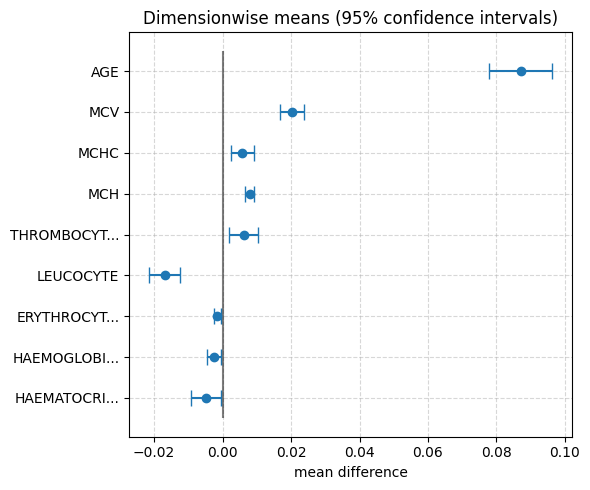
\includegraphics[width=0.7\textwidth]{images/begeat_dimension.png}
    \caption{Dimensionwise Means Difference for BeGreat Model}
    \label{fig:begreat_means_diff}
\end{figure}

From Figure \ref{fig:begreat_means_diff}, Model BeGreat shows small mean differences for most dimensions, with the largest difference observed in AGE. The overall pattern indicates a close match to the original data for most dimensions, suggesting good accuracy in replicating the original data's means.

\begin{figure}[H]
    \centering
    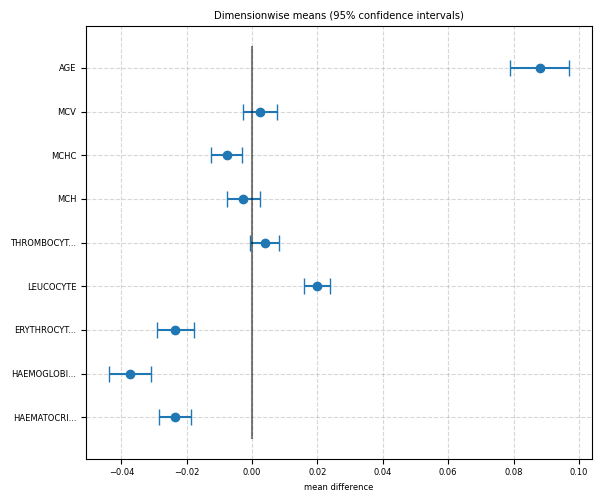
\includegraphics[width=0.7\textwidth]{images/ctgan_dimension.png}
    \caption{Dimensionwise Means Difference for CTGAN Model}
    \label{fig:ctgan_means_diff}
\end{figure}

From Figure \ref{fig:ctgan_means_diff}, Model CTGAN shows small mean differences for most dimensions, but with slightly larger differences in dimensions like AGE and MCV. The overall pattern indicates a reasonable match to the original data for most dimensions, though not as close as BeGreat.

\begin{figure}[H]
    \centering
    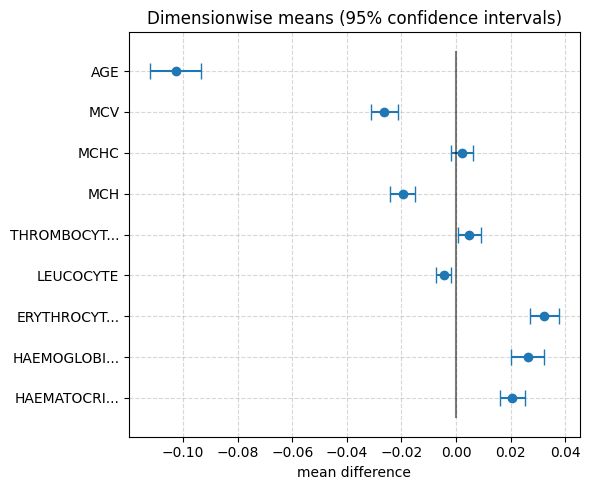
\includegraphics[width=0.7\textwidth]{images/llama_dimension.png}
    \caption{Dimensionwise Means Difference for Llama3 Model}
    \label{fig:llama3_means_diff}
\end{figure}

From Figure \ref{fig:llama3_means_diff}, Model Llama3 shows larger mean differences for several dimensions, particularly AGE, indicating a less accurate replication of the original data's means compared to BeGreat and CTGAN. However, it still demonstrates a reasonable level of accuracy for some dimensions.

\subsection{Summary of Findings}

The dimensionwise means difference plots reveal that:
- **BeGreat** shows the smallest mean differences for most dimensions, indicating the best overall performance in replicating the original data's means.
- **CTGAN** performs reasonably well but shows slightly larger differences in some dimensions compared to BeGreat.
- **Llama3** exhibits larger mean differences for several dimensions, particularly AGE, indicating a lower accuracy in replicating the original data's means.

\subsection{Conclusion}

These findings highlight the strengths and limitations of each model in terms of dimensionwise means difference. The BeGreat model is recommended for applications requiring high fidelity in replicating the original data's means, while the CTGAN model offers a balanced performance. The Llama3 model may require further refinement to improve accuracy in replicating the original data's means.


%--------------------------------------------------------------------------------------------------------------------------------------------------------------------------------------------------------------------



%--------------------------------------------------------------------------------------------------------------------------------------------------------------------------------------------------------------------


%-------------------------------------------------------------------------------------------------------------------------------------------------------------------------------------------------------------------------------------------------------------------------------------------

















% Anaylse the impact of different hyperparameters on data quality and realism.

% Discuss the ethical and societal implications of synthetic data generated using LLMs.
\chapter{Conclusion}

% Summarise the key findings and contributions of the dissertation.

% Emphasise the potential of LLMs for generation high-quality synthetic data in healthcare.

% Discuss the ethical and societal implications of using LLMs for data generation.


% \begin{thebibliography}{refs}                   %% Start your bibliography here; you can
\addcontentsline {toc}{chapter}{Bibliography}     %% Force Bibliography to appear in contents
\bibliographystyle{apalike}
\bibliography{refs}                               %% also use the \bibliography command
%\end{thebibliography}                            %% to generate your bibliography.


\addcontentsline {toc}{chapter}{Appendices}       %% Force Appendices to appear in contents
\begin{appendix}
    \chapter*{TabularToTextualConverter Implementation}
\label{app:tabTotext_appendix}

\begin{verbatim}

import pandas as pd

class TabularToTextualConverter:
    def __init__(self, file_path):
        self.file_path = file_path
        self.data = None
        self.string_list = []

    def read_data(self):
        print("Reading data from:", self.file_path)
        self.data = pd.read_csv(self.file_path)
    
    def transform_rows(self):
        # Check if data is read
        if self.data is None:
            raise ValueError("Data not loaded. Call read_data() first.")
        
        print("Transforming rows...")
        # Iterate over each row in the DataFrame
        for index, row in self.data.iterrows():
            # Create a list to store the key-value pairs
            key_value_pairs = []
            
            # Iterate over each column in the row
            for col_name in self.data.columns:
                key_value_pairs.append(f"{col_name}: {row[col_name]}")
            
            # Join the key-value pairs into a single string
            row_string = ", ".join(key_value_pairs)
            
            # Prepend the patient number and add to the list
            patient_string = f"Patient {index + 1}: [{row_string}]"
            self.string_list.append(patient_string)

    def get_string_list(self):
        return self.string_list

    def get_combined_string(self):
        # Combine the list into a single string
        return ", ".join(self.string_list)

    def print_string_list(self):
        print("Printing string list:")
        for s in self.string_list:
            print(s)

    def print_combined_string(self):
        print("Printing combined string:")
        print(self.get_combined_string())

    def get_subset_data(self, number_of_patients=14):
        # Subdivide the string list into subsets
        print(f"Getting subset data for {number_of_patients} patients...")
        subset_data = []
        
        # Iterate over the string list
        for i in range(0, len(self.string_list), number_of_patients):
            subset_data.append(self.string_list[i:i+number_of_patients])

        return subset_data
        
\end{verbatim}
    \chapter*{Configuration File Implementation}
\label{app:config_implementation}

\begin{verbatim}

[dataset]
data_in_use = data1

[data1]
name = 
data_dir = ../datasets/data.csv
headers = Disease, Fever, Cough, Fatigue, Difficulty Breathing, Age, Gender, Blood Pressure, Cholesterol Level, Outcome Variable
number_of_records = 348

[data2]
name = hospital-triage-and-patient-history-data
data_dir = ../datasets/data2.csv

[data3]
name = 
data_dir = ../datasets/indian_liver_patient.csv

[data4]
name = Patient Treatment Classification
data_dir = ../datasets/data-ori.csv
headers = HAEMATOCRIT, HAEMOGLOBINS, ERYTHROCYTE, LEUCOCYTE, THROMBOCYTE, MCH, MCHC, MCV, AGE, SEX, SOURCE

################################################################################################################




# BeGreat
[begreat]
llm = distilgpt2
batch_size = 64
epochs = 32
save_steps = 400000
n_samples = 4410
#####348
output_file = ./results/synthetic_data_begreat_data_ori.csv
output_file2 = ./results/synthetic_data_begreat.csv



# CTGAN
[ctgan]
input_file = ./results/synthetic_data_ctgan_data_ori.txt
input_file2 = ./results/synthetic_data_ctgan.txt
output_file = ./results/synthetic_data_ctgan_data_ori.csv
output_file2 = ./results/synthetic_data_ctgan.csv
#discrete_columns = Disease, Fever, Cough, Fatigue, Difficulty Breathing, Gender, Blood Pressure, Cholesterol Level, Outcome Variable
discrete_columns = HAEMATOCRIT, HAEMOGLOBINS, ERYTHROCYTE, LEUCOCYTE, THROMBOCYTE, MCH, MCHC, MCV, AGE, SEX, SOURCE
num_samples = 4410
#####348


# Google Gemma
[gemma-2b]
input_file = ./results/synthetic_data_gemma_2b.txt
input_file2 = ./results/synthetic_data_gemma_2b_large.txt
output_file = ./results/synthetic_data_gemma_2b.csv
output_file2 = ./results/synthetic_data_gemma_2b_large.csv

[gemma-7b]
input_file = ./results/synthetic_data_gemma_7b.txt
input_file2 = ./results/synthetic_data_gemma_7b_large.txt
output_file = ./results/synthetic_data_gemma_7b.csv
output_file2 = ./results/synthetic_data_gemma_7b_large.csv

[gemma2-9b]
input_file = ./results/synthetic_data_gemma2_9b.txt
output_file = ./results/synthetic_data_gemma2_9b.csv
input_text_11 = " Generate 12 additional patient records in the following format:\
                            Disease: disease, Fever: fever, Cough: cough, Fatigue: fatigue, Difficulty Breathing: difficulty_breathing, Age: age, Gender: gender, Blood Pressure: blood_pressure, Cholesterol Level: cholesterol_level, Outcome Variable: outcome\
                            Use this current data for reference:\
                            "
input_text_1 = "Generate 15 patient records using the following data as reference:\
                And put the data in the following format:\
                Patient i:
                HAEMATOCRIT: 31.5, HAEMOGLOBINS: 10.4, ERYTHROCYTE: 3.15, LEUCOCYTE: 9.1, THROMBOCYTE: 187, MCH: 33.0, MCHC: 33.0, MCV: 100.0, AGE: 98, SEX: F, SOURCE: in\
                Data:"



# Meta LLaMa 2
[llama-2-7b]
input_file = ./results/synthetic_data_llama_2_7b.txt
input_file2 = ./results/synthetic_data_llama_2_7b_large.txt
output_file = ./results/synthetic_data_llama_2_7b.csv
output_file2 = ./results/synthetic_data_llama_2_7b_large.csv
input_text = "Generate 12 additional patient records in the following format and don't hesitate to generate new diseases as well:\
                Patient i: [Disease: disease, Fever: fever, Cough: cough, Fatigue: fatigue, Difficulty Breathing: difficulty_breathing, Age: age, Gender: gender, Blood Pressure: blood_pressure, Cholesterol Level: cholesterol_level, Outcome Variable: outcome]\
                Use this current data for reference:\
                Data: "

[llama-2-70b]
input_file = ./results/synthetic_data_llama_2_70b.txt
input_file2 = ./results/synthetic_data_llama_2_70b_large.txt
output_file = ./results/synthetic_data_llama_2_70b.csv
output_file2 = ./results/synthetic_data_llama_2_70b_large.csv


# Meta LLaMa 3
[llama-3-8b]
#input_text = "Generate 12 additional patient records in the following format and don't hesitate to generate new diseases as well:\
                    #Patient i: [Disease: disease, Fever: fever, Cough: cough, Fatigue: fatigue, Difficulty Breathing: difficulty_breathing, Age: age, Gender: gender, Blood Pressure: blood_pressure, Cholesterol Level: cholesterol_level, Outcome Variable: outcome]\
                    #Use this current data for reference:\
                    #Data: "
input_text = "Generate 11 additional patient records in the following format and don't hesitate to generate new diseases as well:\
                    Patient i: [Age: age, Gender: gender, Total Bilirubin: total_bilirubin, Direct Bilirubin: direct_bilirubin,
                    Alkaline Phosphotase: alkaline_phosphotase, Alamine Aminotransferase: alamine_aminotransferase,
                    Aspartate Aminotransferase: aspartate_aminotransferase, Total Proteins: total_proteins,
                    Albumin: albumin, Albumin and Globulin Ratio: albumin_and_globulin_ratio]\
                    Use this current data for reference:\
                    Data: "

input_text_ = "Generate 15 patient records using the following data as reference:\
                And put the data in the following format:\
                Patient i:
                HAEMATOCRIT: 31.5, HAEMOGLOBINS: 10.4, ERYTHROCYTE: 3.15, LEUCOCYTE: 9.1, THROMBOCYTE: 187, MCH: 33.0, MCHC: 33.0, MCV: 100.0, AGE: 98, SEX: F, SOURCE: in\
                Data:"

input_file2 = ./results/synthetic_data_llama_3_8b_data_ori.txt
input_file = ./results/synthetic_data_llama_3_8b.txt
output_file2 = ./results/synthetic_data_llama_3_8b_data_ori.csv
output_file = ./results/synthetic_data_llama_3_8b.csv
pattern = Patient \d+: \[Disease: (.*?), Fever: (.*?), Cough: (.*?), Fatigue: (.*?), Difficulty Breathing: (.*?), Age: (\d+), Gender: (.*?), Blood Pressure: (.*?), Cholesterol Level: (.*?), Outcome Variable: (.*?)\]
#pattern = r"Patient \d+:\s*HAEMATOCRIT: (.*?), HAEMOGLOBINS: (.*?), ERYTHROCYTE: (.*?), LEUCOCYTE: (.*?), THROMBOCYTE: (.*?), MCH: (.*?), MCHC: (.*?), MCV: (.*?), AGE: (\d+), SEX: (.*?), SOURCE: (.*?)\n"
#pattern = \b(HAEMATOCRIT|HAEMOGLOBINS|ERYTHROCYTE|LEUCOCYTE|THROMBOCYTE|MCH|MCHC|MCV|AGE|SEX|SOURCE):\s*([^,]+)

[llama-3-70b]
input_file = ./results/synthetic_data_llama_3_70b.txt
input_file2 = ./results/synthetic_data_llama_3_70b_large.txt
output_file = ./results/synthetic_data_llama_3_70b.csv
output_file2 = ./results/synthetic_data_llama_3_70b_large.csv


# Mistral 7b
[mistral-7b]
input_text = "Generate 12 additional patient records in the following format and don't hesitate to generate new diseases and avoid same patients as in the provided data:\
                    Patient i: [Disease: disease, Fever: fever, Cough: cough, Fatigue: fatigue, Difficulty Breathing: difficulty_breathing, Age: age, Gender: gender, Blood Pressure: blood_pressure, Cholesterol Level: cholesterol_level, Outcome Variable: outcome]\
                    Use this current data for reference:\
                    Data: "
input_file = ./results/synthetic_data_mistral-7b.txt
input_file2 = ./results/synthetic_data_mistral-7b_large.txt
output_file = ./results/synthetic_data_mistral-7b.csv
output_file2 = ./results/synthetic_data_mistral-7b_large.csv



\end{verbatim}
    \chapter*{CTGAN Implementation}
\label{app:ctganimplementation}

\begin{verbatim}

from ctgan import CTGAN
import pandas as pd
import configparser

CONFIG_FILE = "../config.ini"

class SyntheticDataGeneratorCTGAN:
    def __init__(self, epochs=32):
        self.ctgan = CTGAN(epochs=epochs)
        print("Reading configuration file...")
        config = configparser.ConfigParser()
        config.read(CONFIG_FILE)
        self.output_file = config['ctgan']['output_file']
        dataset = config['dataset']['data_in_use']
        self.data = pd.read_csv(config[dataset]['data_dir'])
        self.discrete_columns = config['ctgan']['discrete_columns'].split(', ')
        self.num_samples = int(config['ctgan']['num_samples'])
    
    def fit_and_generate(self):
        print("Fitting the data using CTGAN...")
        self.ctgan.fit(self.data, self.discrete_columns)
        synthetic_data = self.ctgan.sample(self.num_samples)
        synthetic_data.to_csv(self.output_file, index=False)
        print("Synthetic data generated and saved to", self.output_file)

# Measure the convergence


generator = SyntheticDataGeneratorCTGAN(epochs=32)
generator.fit_and_generate()

\end{verbatim}
    \chapter*{BeGreat Implementation}
\label{app:begreat_implementation}

\begin{verbatim}

from be_great import GReaT
import pandas as pd
import configparser

CONFIG_FILE = "../config.ini"

class SyntheticDataGeneratorBeGreat:
    def __init__(self):
        print("Reading configuration file...")
        config = configparser.ConfigParser()
        config.read(CONFIG_FILE)

        self.llm = str(config['begreat']['llm'])
        self.batch_size = int(config['begreat']['batch_size'])
        self.epochs = int(config['begreat']['epochs'])
        self.save_steps = int(config['begreat']['save_steps'])
        dataset = config['dataset']['data_in_use']
        self.data = pd.read_csv(config[dataset]['data_dir'])
        self.n_samples = int(config['begreat']['n_samples']) 
        self.output_file = config['begreat']['output_file']

        self.model = GReaT(llm=self.llm, batch_size=self.batch_size, epochs=self.epochs, save_steps=self.save_steps)


    def fit(self):
        print("Fitting the model to the data...")
        self.model.fit(self.data)
    
    def generate_samples(self):
        print("Generating synthetic data...")
        synthetic_data = self.model.sample(n_samples=self.n_samples)
        return synthetic_data
    
    def save_samples(self, synthetic_data):
        synthetic_data.to_csv(self.output_file, index=False)
        print(f"Synthetic data generated and saved to {self.output_file}")

\end{verbatim}
    \chapter*{LLaMa-3 File Implementation}
\label{app:llama_implementation}

\begin{verbatim}

# Copyright (c) Meta Platforms, Inc. and affiliates.
# This software may be used and distributed in accordance with the terms of the Llama 3 Community License Agreement.

from typing import List, Optional
import fire
import sys
import TabularToTextualConverter as TabularToTextualConverter
import TextualToTabularConverter as TextualToTabularConverter
import os
import configparser

sys.path.append("./llama3")
from llama import Dialog, Llama


CONFIG_FILE = "../config.ini"

def main(
    ckpt_dir: str,
    tokenizer_path: str,
    temperature: float = 0.6,
    top_p: float = 0.9,
    max_seq_len: int = 512,
    max_batch_size: int = 4,
    max_gen_len: Optional[int] = None,
):
    """
    Examples to run with the models finetuned for chat. Prompts correspond of chat
    turns between the user and assistant with the final one always being the user.

    An optional system prompt at the beginning to control how the model should respond
    is also supported.

    The context window of llama3 models is 8192 tokens, so `max_seq_len` needs to be <= 8192.

    `max_gen_len` is optional because finetuned models are able to stop generations naturally.
    """

    print("Reading configuration file...")
    config = configparser.ConfigParser()
    config.read(CONFIG_FILE)
    dataset = config['dataset']['data_in_use']
    data = config[dataset]['data_dir']

    print("Formatting patient data...")
    patient_data_formatter = TabularToTextualConverter.TabularToTextualConverter(data)
    patient_data_formatter.read_data()
    patient_data_formatter.transform_rows()
    #combined_string = patient_data_formatter.get_combined_string()

    subset_data = patient_data_formatter.get_subset_data(number_of_patients=11)

    print("Building Llama generator...")
    generator = Llama.build(
        ckpt_dir=ckpt_dir,
        tokenizer_path=tokenizer_path,
        max_seq_len=max_seq_len,
        max_batch_size=max_batch_size,
    )

    i = 0

    input_text = config['llama-3-8b']['input_text']

    while i < len(subset_data):
        print("Generating patient records... number: " + str(i))
        dialogs: List[Dialog] = [
            [{"role": "user", "content": input_text +  str(subset_data[i])}],
        ]

        results = generator.chat_completion(
            dialogs,
            max_gen_len=max_gen_len,
            temperature=temperature,
            top_p=top_p,
        )

        print("Printing generated records...")
        """
        for dialog, result in zip(dialogs, results):
            for msg in dialog:
                print(f"{msg['role'].capitalize()}: {msg['content']}\n")
            print(
                f"> {result['generation']['role'].capitalize()}: {result['generation']['content']}"
            )
            print("\n==================================\n")
        """
        
        results_txt = config['llama-3-8b']['input_file']

        # Check if the file exists
        if not os.path.exists(results_txt):
            # Create the file if it doesn't exist
            with open(results_txt, 'w') as f:
                pass

        # Store the results in a txt file
        print("Storing the results in txt file...")
        lines_to_skip = ["User:", "Use", "Data:", "> Assistant:", "Note:", "Patient i:", "Note that", "Let me", "And put the data"]

        def filter_lines(text: str, prefixes: List[str]) -> str:
            filtered_lines = []
            for line in text.splitlines():
                if not any(line.startswith(prefix) for prefix in prefixes):
                    filtered_lines.append(line)
            return "\n".join(filtered_lines)

        with open(results_txt, 'a') as f:
            for dialog, result in zip(dialogs, results):
                dialog_content = "\n".join([f"{msg['role'].capitalize()}: {msg['content']}" for msg in dialog])
                result_content = f"> {result['generation']['role'].capitalize()}: {result['generation']['content']}"
                combined_content = dialog_content + "\n" + result_content
                
                filtered_content = filter_lines(combined_content, lines_to_skip)
                
                f.write(filtered_content + "\n\n")

        i += 1
        


    print("Converting generated text to tabular format...")
    converter = TextualToTabularConverter.TextualToTabularConverter(CONFIG_FILE)
    converter.process()

if __name__ == "__main__":
    fire.Fire(main)


\end{verbatim}

    \chapter*{TextualToTabularConverter Implementation}
\label{app:textTotab_appendix}

\begin{verbatim}

"""
import csv
import re
import configparser

class TextualToTabularConverter:
    def __init__(self, config_file):
        self.config_file = config_file
        self.config = configparser.ConfigParser()
        self.config.read(self.config_file)
        self.input_file = self.config['llama-3-8b']['input_file']
        self.output_file = self.config['llama-3-8b']['output_file']
        self.data = ""
        self.matches = []
        data_in_use = self.config['dataset']['data_in_use']
        self.headers = self.config[data_in_use]['headers'].split(', ')
        self.pattern = re.compile(self.config['llama-3-8b']['pattern'], re.MULTILINE)

    def read_data(self):
        print("Reading data from:", self.input_file)
        with open(self.input_file, 'r') as file:
            self.data = file.read()

    def parse_data(self):
        print("Parsing data...")
        # Remove any unwanted text
        self.data = re.sub(r'HAEMATOCRIT: \d+\.\d+"', '', self.data)
        
        # Extract individual patient data blocks
        patient_blocks = re.split(r'\nPatient \d+:\n', self.data)
        for block in patient_blocks:
            block = block.strip()
            if block:
                # Extract the values using the headers
                match = [self.extract_value(block, header) for header in self.headers]
                self.matches.append(match)

    def extract_value(self, block, header):
        # Use regex to extract the value corresponding to the header
        pattern = re.compile(rf'{header}:\s*([^,\n]+)')
        match = pattern.search(block)
        if match:
            return match.group(1).strip()
        return ""

    def write_csv(self):
        print("Writing CSV to:", self.output_file)
        with open(self.output_file, 'w', newline='') as csvfile:
            writer = csv.writer(csvfile)
            writer.writerow(self.headers)
            for match in self.matches:
                # Handle potential trailing backslash
                cleaned_match = [value.rstrip('\\') for value in match]
                writer.writerow(cleaned_match)

    def process(self):
        print("Starting data processing...")
        self.read_data()
        self.parse_data()
        self.write_csv()
        print("Data processing complete.")
"""

import csv
import re
import configparser

class TextualToTabularConverter:
    def __init__(self, config_file):
        self.config_file = config_file
        self.config = configparser.ConfigParser()
        self.config.read(self.config_file)
        self.input_file = self.config['llama-3-8b']['input_file']
        self.output_file = self.config['llama-3-8b']['output_file']
        self.data = ""
        self.matches = []
        self.headers = ['Disease', 'Fever', 'Cough', 'Fatigue', 'Difficulty Breathing', 'Age', 'Gender', 'Blood Pressure', 'Cholesterol Level', 'Outcome Variable']
        self.pattern = re.compile(
            r'Patient \d+: \[Disease: (.*?), Fever: (.*?), Cough: (.*?), Fatigue: (.*?), Difficulty Breathing: (.*?), Age: (\d+), Gender: (.*?), Blood Pressure: (.*?), Cholesterol Level: (.*?), Outcome Variable: (.*?)\]'
        )

    def read_data(self):
        print("Reading data from:", self.input_file)
        with open(self.input_file, 'r') as file:
            self.data = file.read()

    def parse_data(self):
        print("Parsing data...")
        self.matches = self.pattern.findall(self.data)

    def write_csv(self):
        print("Writing CSV to:", self.output_file)
        with open(self.output_file, 'w', newline='') as csvfile:
            writer = csv.writer(csvfile)
            writer.writerow(self.headers)
            for match in self.matches:
                writer.writerow(match)

    def process(self):
        print("Starting data processing...")
        self.read_data()
        self.parse_data()
        self.write_csv()
        print("Data processing complete.")

\end{verbatim}
\end{appendix}




\end{document}                                    %% END THE DOCUMENT
